%%
%% This is file `sample-sigconf.tex',
%% generated with the docstrip utility.
%%
%% The original source files were:
%%
%% samples.dtx  (with options: `sigconf')
%% 
%% IMPORTANT NOTICE:
%% 
%% For the copyright see the source file.
%% 
%% Any modified versions of this file must be renamed
%% with new filenames distinct from sample-sigconf.tex.
%% 
%% For distribution of the original source see the terms
%% for copying and modification in the file samples.dtx.
%% 
%% This generated file may be distributed as long as the
%% original source files, as listed above, are part of the
%% same distribution. (The sources need not necessarily be
%% in the same archive or directory.)
%%
%% The first command in your LaTeX source must be the \documentclass command.
\documentclass[sigconf]{acmart}

\usepackage{latexsym}
\usepackage{makecell}
\usepackage[english]{babel}
\usepackage{ulem}

%%
%% \BibTeX command to typeset BibTeX logo in the docs
\AtBeginDocument{%
  \providecommand\BibTeX{{%
    \normalfont B\kern-0.5em{\scshape i\kern-0.25em b}\kern-0.8em\TeX}}}

%% Rights management information.  This information is sent to you
%% when you complete the rights form.  These commands have SAMPLE
%% values in them; it is your responsibility as an author to replace
%% the commands and values with those provided to you when you
%% complete the rights form.
\setcopyright{acmcopyright}
\copyrightyear{2021}
\acmYear{2021}
\setcopyright{iw3c2w3}
\acmConference[WWW '21]{Proceedings of the Web Conference 2021}{April 19--23, 2021}{Ljubljana, Slovenia}
\acmBooktitle{Proceedings of the Web Conference 2021 (WWW '21), April 19--23, 2021, Ljubljana, Slovenia}
\acmPrice{}
\acmDOI{10.1145/3442381.3449876}
\acmISBN{978-1-4503-8312-7/21/04}
%%
%% Submission ID.
%% Use this when submitting an article to a sponsored event. You'll
%% receive a unique submission ID from the organizers
%% of the event, and this ID should be used as the parameter to this command.
%%\acmSubmissionID{123-A56-BU3}

%%
%% The majority of ACM publications use numbered citations and
%% references.  The command \citestyle{authoryear} switches to the
%% "author year" style.
%%
%% If you are preparing content for an event
%% sponsored by ACM SIGGRAPH, you must use the "author year" style of
%% citations and references.
%% Uncommenting
%% the next command will enable that style.
%%\citestyle{acmauthoryear}

%%
%% end of the preamble, start of the body of the document source.
\begin{document}

%%
%% The "title" command has an optional parameter,
%% allowing the author to define a "short title" to be used in page headers.
\title{Diverse and Specific Clarification Question Generation with Keywords}

%%
%% The "author" command and its associated commands are used to define
%% the authors and their affiliations.
%% Of note is the shared affiliation of the first two authors, and the
%% "authornote" and "authornotemark" commands
%% used to denote shared contribution to the research.

\author{Zhiling Zhang}
\affiliation{%
  \institution{Shanghai Jiao Tong University}
  \city{Shanghai}
  \country{China}}
\email{blmoistawinde@sjtu.edu.cn}
\orcid{0000-0002-8081-704X}

\author{Kenny Q. Zhu}
\affiliation{%
  \institution{Shanghai Jiao Tong University}
  \city{Shanghai}
  \country{China}}
\email{kzhu@cs.sjtu.edu.cn}
\authornote{Corresponding author.}
%%
%% By default, the full list of authors will be used in the page
%% headers. Often, this list is too long, and will overlap
%% other information printed in the page headers. This command allows
%% the author to define a more concise list
%% of authors' names for this purpose.
%\renewcommand{\shortauthors}{Zhang and Zhu}

%%
%% The abstract is a short summary of the work to be presented in the
%% article.
\begin{abstract}
  Product descriptions on e-commerce websites often suffer from 
missing important aspects. \textit{Clarification question generation} (CQGen) can be a promising approach to help alleviate the problem. Unlike traditional QGen assuming the existence of answers in the context and generating questions accordingly, CQGen mimics user behaviors of asking for unstated information. The generated CQs can serve as a sanity check or proofreading to help e-commerce 
merchant to identify potential missing information before advertising their
product, and improve consumer experience consequently. 
Due to the variety of possible user backgrounds and use cases, 
the information need can be quite diverse but also specific to a detailed
topic, while previous works assume generating one CQ per context and 
the results tend to be generic. We thus propose the task 
of \textit{Diverse CQGen} and also tackle the challenge of specificity. 
We propose a new model named \textit{KPCNet}, which generates CQs with 
Keyword Prediction and Conditioning, to deal with the tasks. 
Automatic and human evaluation on 2 datasets (\texttt{Home \& Kitchen}, 
\texttt{Office}) showed that KPCNet can generate more specific questions 
and promote better group-level diversity than several competing baselines. \footnote{Our code is available at \url{https://github.com/blmoistawinde/KPCNet}}
\end{abstract}

%%
%% Keywords. The author(s) should pick words that accurately describe
%% the work being presented. Separate the keywords with commas.
\keywords{clarification question, text generation, diverse generation, keyword prediction, e-commerce}

%%
%% This command processes the author and affiliation and title
%% information and builds the first part of the formatted document.
\maketitle

%\IEEEraisesectionheading{
% %\IEEEraisesectionheading{
% %\IEEEraisesectionheading{
% \input{intro}
\section{Introduction}\label{sec:intro}
 %}
% \section{Introduction}\label{sec:intro}

% \begin{enumerate}
% \item Motivation: application scenarios (with 1-2 running examples);
% \item Characteristics of the data sources and their challenges;
% \item Briefly introduce previous approaches to extract information 
% from images including setting the document zone, and their limitations.
% \item General flow of our approach (may give a diagram here)
% \end{enumerate}
% scenary

Due to ever evolving hardware and software, many medical images
such as electro-cardio graphs (ECGs), X-ray or ultrasound images  
are directly printed and stored in hard copy formats. 
% \KZ{Insert 4 example images here.}
%Examples are shown in \figref{fig:medicalImages}. 
% These images often contain a mix of graphics and text, which
% include parameter settings of the hardware, test measurements or simple
% diagnosis. 
These images often contain a mix of graphics and text, which 
include technical settings of the hardware used, test measurements or simple diagnoses.
Recently, there has been a growing demand for digitizing such 
medical information from paper media sources, especially legacy ones, or patients who want to keep track of these documents by themselves digitally. 
Apart from scanning the graphics into a digital format, extracting 
the semi-structured textual information is also an important part of
building electronic medical records for patients. 

%\begin{figure}[!htb]
%\centering
%\subfloat[ECG]{
%\label{fig:medicalimage:ecg}
%\epsfig{file=figure/17_ori.eps, width=0.4\columnwidth}
%}
%% \hfill
%\subfloat[MRI]{
%	\label{fig:medicalimage:mrt}
%	\epsfig{file=figure/MRI.eps, width=0.4\columnwidth}
%}
%\\
%\subfloat[X-RAY]{
%\label{fig:medicalimage:xray}
%\epsfig{file=figure/X-RAY.eps, width=0.4\columnwidth}
%}
%%\hfill
%\subfloat[EEG]{
%\label{fig:medicalimage:eeg}
%\epsfig{file=figure/EEG.eps, width=0.4\columnwidth}
%}
%\caption{Examples of Medical Images}
%\label{fig:medicalImages}
%\end{figure}

Optical character recognition (OCR)  \cite{mori1992historical,smith2007overview} is 
a traditional technique used to turn images of printed text into machine encoded
text. It is well researched and performs well on plain text 
documents such as novels and reports, for a variety of languages. 
%For example, Tesseract, which is one of 
%the most popular open source multilingual recognizers, logs an error 
%rate of 3.72\% for English words and 3.77\% for simplified 
%Chinese characters\cite{smith2009adapting}. 
%Google Books \cite{googlebooks} and Gutenberg \cite{gutenberg} are
%projects which have scanned a large number of paper books into text for free and open
%access. These projects made exclusive use of OCR for this conversion and 
%achieved high accuracy \cite{vincent2007google} \cite{lebert2008project}. 
% 99\% for Gutenberg project \cite{lebert2008project}. 
% \KZ{Give the accuracy of google and gutenberg if available.}


\begin{figure}[th]
\centering
\epsfig{file=figure/17_b.eps, width=0.8\columnwidth}
\caption{An ECG image with text area (red circle) of interest.}
\label{fig:ecgexample2}
\end{figure}

For a semi-structured medical image, such as 
\figref{fig:ecgexample2}, we would like to extract the attribute-value 
pairs (e.g., {\em Vent. rate = 63 bpm}) and possibly other values such as
date ({\em 18-Nov-2010}) and time ({\em 9:13:02}) since those values endow us with lots of information about the patient. 
Existing OCR software cannot extract such structured information in a straightforward 
fashion, 
but instead it produces rather convoluted results from the whole image, 
similar to those in \figref{fig:ocrre}, which was produced by Tesseract, 
a popular multi-lingual recognizers. 
% \KZ{Maybe include the x-y coordinate info in the output as well?}  

\begin{figure}[th]
\centering
\scriptsize
\begin{verbatim}
<p class="ocr_par" title="box 263 33 444 119">
   <span class="ocr_l" title="box 264 33 336 45">
       <span class="ocrx_w" title="box 264 33 299 45">Vcnt.</span> 
       <span class="ocrx_w" title="box 308 34 336 45">rule</span> 
   </span>
   <span class='ocr_l'>
       <span class="ocrx_w" title="box 264 51 283 64">PR</span> 
       <span class="ocrx_w" title="box 291 51 346 64">Interval</span> 
       <span class="ocrx_w" title="box 389 52 411 64">140</span> 
       <span class="ocrx_w" title="box 420 55 439 64">ms</span> 
   </span>
   ...
   </span>
</p>
<p class="ocr_p" dir="ltr">
   <span class="ocr_l">
       <span class="ocrx_w" title="box 396 33 411 45">53</span> 
       <span class="ocrx_w" title="box 420 33 449 48">bpm</span> 
   </span>
</p>
\end{verbatim}
\caption{Snippet OCR results in XML, input to our framework.}
\label{fig:ocrre}
\end{figure}


%\input{xmlre1}

%However, OCR alone does not work well on semi-structured text and hence
%can't be directly used for information extraction from the aforementioned
%medical images. \KZ{Give the reason here, perhaps because OCR models are
%largely Markov based? So semi-structured data breaks the flow of text.}
%When a medical image is input to an ordinary OCR software, the spatial 
%information of the text components is often lost or mixed with noises
%and errors.
%%The reason is OCR converts the whole images into text data, in which 
%%useful information often mix with noises and errors. 
%In this paper, we would like to extract the attribute-value pairs
%and possibly other values from \figref{fig:ecgexample1} 
%and \figref{fig:ecgexample2}. 
%% or medical ultrasonography report. 
%Such images contain lots of non-textual information or noises.

% example & ref
%\begin{figure}[ht]
%\centering
%\epsfig{file=figure/46.eps, width=0.8\columnwidth}
%\caption{ECG Images From Printer1}
%\label{fig:ecgexample1}
%\end{figure}

% \begin{figure}[ht]
% \centering
% \subfloat[Printer1]{
% \label{fig:ecgexample:a}
% \epsfig{file=figure/46.eps, width=0.48\columnwidth}
% }
% \hfill
% \subfloat[Printer2]{
% \label{fig:ecgexample:b}
% \epsfig{file=figure/17.eps, width=0.48\columnwidth}
% }
% \caption{ECG images from two different printers}
% \label{fig:ecgexample}
% \end{figure}

Also, errors in the OCR text \cite{darwish2007error,taghva1996evaluation} will greatly affect the effectiveness 
of other related tasks. Much work has been done to improve the performance of the OCR\cite{kolak2003generative,cesarini1998informys}. However, there are still a number of significant challenges involved in extracting the information from medical images or OCR results in XML form. 

% First, medical images differ from pure text document in that them have 
% layout information. 
First, medical images differ from pure text documents in that 
they contain layout information.
Although most current OCR engines attempt to reproduce the physical 
layout of the text units, 
%(along with X-Y coordinates) and store them 
%in a special format such as XML 
% (\KZ{Better in the previous example})
such spatial
information is approximate and sometimes inaccurate, which is why neighboring
text blocks in \figref{fig:ecgexample2}, such as ``Vent. Rate'' and
``63 bpm'' were not automatically combined into the same XML block, but were 
rather far apart (shown in two different ``classes'') in \figref{fig:ocrre} made by OCR softwares. 
%Even for images produced by the same ECG printer, 
%the XML results can still be very different as 
The spatial layout is sensitive to many factors, such as accidental spots 
on the prints, color and contrast, or the angle of the camera. 
%In this case, solutions for other application domains, for example, the web, 
%are not well suited for information extraction from printed documents \cite{bartoli2014semisupervised}. With such inaccurate
%layout information produced by OCR,
%it is not easy to write a simple wrapper program to extract useful
%data from images, even if the images come from the same printer. 

%Writing a wrapper for each
%individual image would be tedious and counter-productive. Therefore,
%a mechanism that makes use of the spatial locality of the 
%text units in the image and 
%accommodates slight variations in the spatial layout would make the extraction
%more accurate and fault-tolerant.

%For example, \figref{fig:ocrre} is the simplified OCR results for the ECGs in 
%\figref{fig:ecgexample1} and \figref{fig:ecgexample2}. The results are in the XML format and have attritube named {\em class} 
%for layout information. Although these two images share similar format. 
%OCR engine generates different results in that it splits elements that 
%should be in the same line into two lines in the second example. 
%XML is sensitive to the layout results so it's hard to tolerate 
%all the layout results. 
%
% example check the term
% layout of ocr results can be restore, so why OCR engine don't restore the results 
% using the similar methods as we do?
% or the way we handle the layout problem is quite simple

% Delete for TIP
% Second, exiting OCR engines make heavy use of Markov properties such as n-grams
% since they primarily target the transformation of large body of text 
% \cite{kolak2003generative}. 
% % \KZ{Needs some refs here.}
% Unfortunately, the semi-structured texts in medical images are often 
% short and not even written in complete sentences, thus breaking Markov assumption. To make
% matters worse, medical images contain scientific language, which may be
% very different from the training corpora of these OCR engines.
% This explains why we see errors like ``Vcnt'' and ``rule'' 
% in \figref{fig:ocrre}. 
% %can't guarantee a perfect performance, which means 
% %there are errors and noises in the OCR results.
% %Many of them due to the fact that the data are no longer long, continous
% %sentences, thus breaking the Markov assumption made by many OCR algorithms. 
% %In \figref{fig:ocrresub:b}, ``Vent." is misrecognized as ``Vcnt.". 
% Without sufficient contextual information, OCR may also misrecognize a 
% digit as an alphabetic character, or as another similar digit. 
% Furthermore, the mix of text with images and formatting
% lines often confuses the OCR engine, which is more biased toward full
% text images.
% Exact pattern matching, as used in
% traditional information extraction, doesn't work with such noisy OCR output
% as it doesn't tolerate noises or errors in text. 
% %It's hard to autocorrect these errors 
% %because image quality is the most important affecting factor. 
% %The text we are processing can be full of no meaning words or 
% %strange numbers. 
% A fuzzy matching strategy is more desirable in this case. 
% % example, what are the traditional IEs

Second, there are many types of medical images, resulting from a variety of
medical tests. Different equipments for the same test can produce vastly 
different images. Writing individual extraction wrappers 
for the OCR outputs of all these formats is tedious and inefficient, 
and difficult for non-programmers.
%not to mention that there are significant programming barriers for 
%writing these wrappers, especially for the medical professionals who are the
%end users of these extraction results. 
%A more user-friendly approach enabling users to specify such extraction requirements would be preferred. 
%There are various kinds of medical images, such as electrocardiograph report, 
%medical ultrasonography report, etc. 
%However the basic measures for each type of medical test (e.g., ECG), 
%are very similar from machine to machine. Only the layouts are 
%different. 
% example medical images

Finally, most off-the-shelf OCR programs are pre-trained with specific 
recognition models, which may not be suitable for the extraction of 
%medical images.
%Furthermore, changes in imaging equipment technology over time may produce 
%different formats, layout, or terminology, rendering existing OCR models 
%obsolete. 
Re-training the models requires a large amount of labeled data, which may
not be available. 
%Incremental training as more labeled data arrives
%is currently not supported by any OCR product.    

%There have been some limited attempts to address some of the above challenges. 
%One solution is a plugin of an OCR program that allows the user to specify 
%target zones of interest in the image to be extracted. The zones specified for
%one image can be applied to images with slight variations by adjusting against
%a fixed reference point that is supposed to exist in all these images.
%% \KZ{I think the problem is not so much with the zones, because we also
%% have zones, but rather with the reference point.}
%% \JY{}
%% example products
%% http://www.square-9.com/automated-data-extraction-optical-character-recognition
%The problem with this solution is its high reliance on the OCR zones  
%established by the user. The performance of the results is affected by the 
%accuracy of the zones. If the zones are too big, the results will be full of 
%noise. If the zones are too small, results will miss something. 
%
%Another solution involves using the page layout analysis technique. The page layout 
%analysis technique is used to determine where the text 
%resides on a page \cite{o1993document}, 
%% \KZ{This page layout analysis approach is not clearly described. I don't understand after reading this paragraph.}
%% By using page layout analysis technique, the hierarchy of physical components 
%% can be generated and to match with the hierarchy of logical components, which 
%% is predefined. 
%this includes identifying and categorizing the 
%regions of interest in the scanned image of a text document. 
%Typically, the first step is to segment text zones from 
%non-textual zones and arrange them in their original order. 
%Then in order to analyze the logical roles of the text zones 
%(titles, captions, footnotes, etc.), logical layout analysis 
%is used for labeling the semantics of the text zones.
%Generally, page layout analysis is used for documents. The problem with applying 
%such a technique on medical images is that it creates so much noises 
%that performance is ultimately affected. 
%For medical imaging reports like ECG, useful information is often 
%found in the small components of the image, while most of the images are 
%read as noises. 
% check paper and more description, weakness, ref

%In this paper, 
%we propose a spatial data description language, which borrows its syntax from
%PADS \cite{fisher+:pads}, an ad hoc data processing language, 
%for describing semi-structured data in medical images. 
%% ref
%We call this language OCR description language, or ODL. 
%ODL is designed for extracting and parsing semi-structured text data 
%from images. We believe that  information extraction from those data in ODL form may be much easier than extracting information from rough data or data in XML form, which means that our preprocessing part proves to be necessary.
%%An example ODL description for the image in 
%%\figref{fig:ecgexample2} is shown in 
%%\figref{fig:description}. \KZ{Make this description two column, and give
%%some brief explanation of this description here.} 
%%The parsing result of this description is shown
%%in \figref{fig:parsing result}. \KZ{Give some explanation of the results,
%%otherwise don't show the result here. E.g., you need to explain what F, E, etc.
%%mean. You want to say that even though rate has been recognized as rule,
%%the bpm value was still extracted (but still wrong!).}
%% \KZ{I removed the preprocessing part, cos it's not important. Talk about it in
%% discussion sec.}
%%The our approach starts by preprocessing the images for text results.
%To use this framework, the user first describes the components in the image
%that he or she is interested in extracting. This includes constant strings
%and variables of different data types.   
%ODL allows the user to specify the approximate spatial layout and constraints on
%the data, e.g., integers within 
%a certain range, real numbers with certain decimal points, etc. 
%%This information is then as the key component in our fuzzy matching strategy. 
%The system then automatically generates a parser for these medical images.
%This parser uses the output XML from OCR with spatial information as an input, 
%and outputs a data structure with values extracted for each variables
%in the description, unless there is an unrecoverable error during the parsing process.
%In addition, approximate layout information and constraints are used in parsing process 
%to tolerate noises and small format variations in the input images. 
%%Specifically, this method could be called fuzzy matching, meaning that more candidates could be saved after the parsing process.  It's obvious that we may have a higher probability to obtain the accurate result if more candidates are kept so that fuzzy match should be used properly in our system.
%%An autogenerated parser based on the ODL description can release us from 
%%repetitive work. In this way, we turn the task of writing complex parsers 
%%into describing information on images.
%
%
%When users process many images of the same format, the system 
%automatically discovers parsing errors given the current model and 
%prompts the user to manually correct some of the frequent and prominent
%errors, which effectively serves as an online labeling function. 
%These incrementally labeled data are then used to update the parsing model. 


%It should be emphasized that the incremental learning model is very important in our whole system. Incremental learning is a machine learning paradigm where the learning process takes place whenever we have new examples or data added to our baisc data set, leading to a most striking difference between incremental learning and traditional machine learning: it does not assume the availability of a sufficient training set before the learning process. What incremental learning in our system is really impressive: it does not require a relatively good and stable training set at first time. In fact, it could improve the parsing result with even relatively rough training sets at first by absorbing new data or corrective information as time passes in dynamic systems. Besides, the process would be very effective when there are some new images coming in since training process would not learn from scratch, which might waste time and computation resource.

%At last, we propose an incrementally human correction framwork which can 
%make the best use of human correction to handle the misrecognition problem. 
% Base on our experiments on about 500 real life ECG images, 
% our approach achieves p1 and p2 after p3 times human correction. 
% experimental results

% \begin{figure}[h]
% \begin{lstlisting}
% Oenum str_month_t{
% 	"Jan", "Feb", "Mar", "Apr",
% 	"May", "Jun", "Jul", "Aug",
% 	"Sept", "Oct", "Nov", "Dec"
% };

% Ounion month_t{
% 	Oint(1,12)	num;
% 	str_month_t	str;
% };

% Ostruct time_t{
% 	Oint(1,31)	day;
% 	"-";
% 	month_t	month;
% 	"-";
% 	Oint	year;
% };

% Ostruct triple_t{
% 	"Vent.";
% 	hskip(\s)	skip1;
% 	"rate";
% 	Oint x;
% 	"bpm";
% 	vskip(\n)	skip2;
% };

% Oscource Ostruct entry_t{
% 	time_t(<-,-,-,0.3l>) t;
% 	triple_t(<0.1w,-,0.5w,->) d;
% };
% \end{lstlisting}
% \caption{Description}\label{fig:description}
% \end{figure}


In order to solve above problems, We design a system which makes three main contributions:
\begin{enumerate}
\item Based on some previous work on data description language \cite{lamport1986document,taft1999post,fisher+:pads},we design a new declarative spatial data description language called \textit{OCR description language}, or ODL,
which allows users to specify spatial and data constraints in medical 
images(\secref{sec:syntax});
\item We propose a noise-tolerant parser which takes OCR results
the ODL description as input and outputs a data structure with values 
extracted for each variables in the description (\secref{sec:semantics});
\item We propose an incremental manual correction 
framework\cite{von2008recaptcha,zhu2012learnpads++}, which 
takes advantage of user corrections  and improves the productivity
significantly (\secref{sec:correction}).
%To be more specific, the framework improves the traditional machine learning methods by using a incremental learning process to avoid starting from scratch when we are trying to apply human corrections in the system. That means the framework would be more effective than most corrective systems.
\end{enumerate}


\section{Introduction}\label{sec:intro}
 %}
% \section{Introduction}\label{sec:intro}

% \begin{enumerate}
% \item Motivation: application scenarios (with 1-2 running examples);
% \item Characteristics of the data sources and their challenges;
% \item Briefly introduce previous approaches to extract information 
% from images including setting the document zone, and their limitations.
% \item General flow of our approach (may give a diagram here)
% \end{enumerate}
% scenary

Due to ever evolving hardware and software, many medical images
such as electro-cardio graphs (ECGs), X-ray or ultrasound images  
are directly printed and stored in hard copy formats. 
% \KZ{Insert 4 example images here.}
%Examples are shown in \figref{fig:medicalImages}. 
% These images often contain a mix of graphics and text, which
% include parameter settings of the hardware, test measurements or simple
% diagnosis. 
These images often contain a mix of graphics and text, which 
include technical settings of the hardware used, test measurements or simple diagnoses.
Recently, there has been a growing demand for digitizing such 
medical information from paper media sources, especially legacy ones, or patients who want to keep track of these documents by themselves digitally. 
Apart from scanning the graphics into a digital format, extracting 
the semi-structured textual information is also an important part of
building electronic medical records for patients. 

%\begin{figure}[!htb]
%\centering
%\subfloat[ECG]{
%\label{fig:medicalimage:ecg}
%\epsfig{file=figure/17_ori.eps, width=0.4\columnwidth}
%}
%% \hfill
%\subfloat[MRI]{
%	\label{fig:medicalimage:mrt}
%	\epsfig{file=figure/MRI.eps, width=0.4\columnwidth}
%}
%\\
%\subfloat[X-RAY]{
%\label{fig:medicalimage:xray}
%\epsfig{file=figure/X-RAY.eps, width=0.4\columnwidth}
%}
%%\hfill
%\subfloat[EEG]{
%\label{fig:medicalimage:eeg}
%\epsfig{file=figure/EEG.eps, width=0.4\columnwidth}
%}
%\caption{Examples of Medical Images}
%\label{fig:medicalImages}
%\end{figure}

Optical character recognition (OCR)  \cite{mori1992historical,smith2007overview} is 
a traditional technique used to turn images of printed text into machine encoded
text. It is well researched and performs well on plain text 
documents such as novels and reports, for a variety of languages. 
%For example, Tesseract, which is one of 
%the most popular open source multilingual recognizers, logs an error 
%rate of 3.72\% for English words and 3.77\% for simplified 
%Chinese characters\cite{smith2009adapting}. 
%Google Books \cite{googlebooks} and Gutenberg \cite{gutenberg} are
%projects which have scanned a large number of paper books into text for free and open
%access. These projects made exclusive use of OCR for this conversion and 
%achieved high accuracy \cite{vincent2007google} \cite{lebert2008project}. 
% 99\% for Gutenberg project \cite{lebert2008project}. 
% \KZ{Give the accuracy of google and gutenberg if available.}


\begin{figure}[th]
\centering
\epsfig{file=figure/17_b.eps, width=0.8\columnwidth}
\caption{An ECG image with text area (red circle) of interest.}
\label{fig:ecgexample2}
\end{figure}

For a semi-structured medical image, such as 
\figref{fig:ecgexample2}, we would like to extract the attribute-value 
pairs (e.g., {\em Vent. rate = 63 bpm}) and possibly other values such as
date ({\em 18-Nov-2010}) and time ({\em 9:13:02}) since those values endow us with lots of information about the patient. 
Existing OCR software cannot extract such structured information in a straightforward 
fashion, 
but instead it produces rather convoluted results from the whole image, 
similar to those in \figref{fig:ocrre}, which was produced by Tesseract, 
a popular multi-lingual recognizers. 
% \KZ{Maybe include the x-y coordinate info in the output as well?}  

\begin{figure}[th]
\centering
\scriptsize
\begin{verbatim}
<p class="ocr_par" title="box 263 33 444 119">
   <span class="ocr_l" title="box 264 33 336 45">
       <span class="ocrx_w" title="box 264 33 299 45">Vcnt.</span> 
       <span class="ocrx_w" title="box 308 34 336 45">rule</span> 
   </span>
   <span class='ocr_l'>
       <span class="ocrx_w" title="box 264 51 283 64">PR</span> 
       <span class="ocrx_w" title="box 291 51 346 64">Interval</span> 
       <span class="ocrx_w" title="box 389 52 411 64">140</span> 
       <span class="ocrx_w" title="box 420 55 439 64">ms</span> 
   </span>
   ...
   </span>
</p>
<p class="ocr_p" dir="ltr">
   <span class="ocr_l">
       <span class="ocrx_w" title="box 396 33 411 45">53</span> 
       <span class="ocrx_w" title="box 420 33 449 48">bpm</span> 
   </span>
</p>
\end{verbatim}
\caption{Snippet OCR results in XML, input to our framework.}
\label{fig:ocrre}
\end{figure}


%% \begin{figure}[ht]
% \centering
% \subfigure[]{
% \label{fig:subfig:a}
% \begin{minipage}[b]{0.2\textwidth}
%\newsavebox{\firstlisting}
%\begin{lrbox}{\firstlisting}% Store first listing
%\begin{lstlisting}
%<p class='ocr_par' dir='ltr'>
%   <span class='ocr_line' id='line_2'>
%       <span class='ocrx_word' id='word_6'>Vent.</span>
%       <span class='ocrx_word' id='word_7'>rate</span>
%       <span class='ocrx_word' id='word_8'>65</span>
%       <span class='ocrx_word' id='word_9'>bpm</span>
%   </span>
%   <span class='ocr_line' id='line_3'>
%       <span class='ocrx_word' id='word_14'>PR</span>
%       <span class='ocrx_word' id='word_15'>interval</span>
%       <span class='ocrx_word' id='word_16'>162</span>
%       <span class='ocrx_word' id='word_17'>ms</span>
%   </span>
%    ...
%</p>
%\end{lstlisting}
%\end{lrbox}
% \end{minipage}
% }
% \hspace[1in]
% \subfigure[]{
% % \label{fig:subfig:b}
% % \begin{minipage}[b]{0.2\textwidth}
\newsavebox{\secondlisting}
\begin{lrbox}{\secondlisting}
% \tiny
\begin{lstlisting}[basicstyle=\tiny,]
<p class="ocr_par" title="box 263 33 444 119">
   <span class="ocr_l" title="box 264 33 336 45">
       <span class="ocrx_w" title="box 264 33 299 45">Vcnt.</span>
       <span class="ocrx_w" title="box 308 34 336 45">rule</span>
   </span>
   <span class='ocr_l'>
       <span class="ocrx_w" title="box 264 51 283 64">PR</span>
       <span class="ocrx_w" title="box 291 51 346 64">Interval</span>
       <span class="ocrx_w" title="box 389 52 411 64">140</span>
       <span class="ocrx_w" title="box 420 55 439 64">ms</span>
   </span>
   ...
   </span>
</p>
<p class="ocr_p" dir="ltr">
   <span class="ocr_l">
       <span class="ocrx_w" title="box 396 33 411 45">53</span>
       <span class="ocrx_w" title="box 420 33 449 48">bpm</span>
   </span>
</p>
\end{lstlisting}
\end{lrbox}
% % \end{minipage}
% }

% \KZ{\figref{fig:ocrre} is output from what software? Tesseract?}
\begin{figure*}[th]
%\subfloat[Image From Printer1]{
%\label{fig:ocrresub:a}
%\scalebox{0.8}{\usebox{\firstlisting}}}
%\hfill
%\subfloat[Image From Printer2]{
\scalebox{1.6}{\usebox{\secondlisting}}
% \label{fig:ocrre}
\caption{A fragment of raw OCR results for ECG with layout information.}
%\caption{Simplified OCR Results in XML for an ECG with Layout Information}
%\label{fig:ocrresub:b}
\label{fig:running-xml}
\end{figure*}

% \lipsum[2]


%However, OCR alone does not work well on semi-structured text and hence
%can't be directly used for information extraction from the aforementioned
%medical images. \KZ{Give the reason here, perhaps because OCR models are
%largely Markov based? So semi-structured data breaks the flow of text.}
%When a medical image is input to an ordinary OCR software, the spatial 
%information of the text components is often lost or mixed with noises
%and errors.
%%The reason is OCR converts the whole images into text data, in which 
%%useful information often mix with noises and errors. 
%In this paper, we would like to extract the attribute-value pairs
%and possibly other values from \figref{fig:ecgexample1} 
%and \figref{fig:ecgexample2}. 
%% or medical ultrasonography report. 
%Such images contain lots of non-textual information or noises.

% example & ref
%\begin{figure}[ht]
%\centering
%\epsfig{file=figure/46.eps, width=0.8\columnwidth}
%\caption{ECG Images From Printer1}
%\label{fig:ecgexample1}
%\end{figure}

% \begin{figure}[ht]
% \centering
% \subfloat[Printer1]{
% \label{fig:ecgexample:a}
% \epsfig{file=figure/46.eps, width=0.48\columnwidth}
% }
% \hfill
% \subfloat[Printer2]{
% \label{fig:ecgexample:b}
% \epsfig{file=figure/17.eps, width=0.48\columnwidth}
% }
% \caption{ECG images from two different printers}
% \label{fig:ecgexample}
% \end{figure}

Also, errors in the OCR text \cite{darwish2007error,taghva1996evaluation} will greatly affect the effectiveness 
of other related tasks. Much work has been done to improve the performance of the OCR\cite{kolak2003generative,cesarini1998informys}. However, there are still a number of significant challenges involved in extracting the information from medical images or OCR results in XML form. 

% First, medical images differ from pure text document in that them have 
% layout information. 
First, medical images differ from pure text documents in that 
they contain layout information.
Although most current OCR engines attempt to reproduce the physical 
layout of the text units, 
%(along with X-Y coordinates) and store them 
%in a special format such as XML 
% (\KZ{Better in the previous example})
such spatial
information is approximate and sometimes inaccurate, which is why neighboring
text blocks in \figref{fig:ecgexample2}, such as ``Vent. Rate'' and
``63 bpm'' were not automatically combined into the same XML block, but were 
rather far apart (shown in two different ``classes'') in \figref{fig:ocrre} made by OCR softwares. 
%Even for images produced by the same ECG printer, 
%the XML results can still be very different as 
The spatial layout is sensitive to many factors, such as accidental spots 
on the prints, color and contrast, or the angle of the camera. 
%In this case, solutions for other application domains, for example, the web, 
%are not well suited for information extraction from printed documents \cite{bartoli2014semisupervised}. With such inaccurate
%layout information produced by OCR,
%it is not easy to write a simple wrapper program to extract useful
%data from images, even if the images come from the same printer. 

%Writing a wrapper for each
%individual image would be tedious and counter-productive. Therefore,
%a mechanism that makes use of the spatial locality of the 
%text units in the image and 
%accommodates slight variations in the spatial layout would make the extraction
%more accurate and fault-tolerant.

%For example, \figref{fig:ocrre} is the simplified OCR results for the ECGs in 
%\figref{fig:ecgexample1} and \figref{fig:ecgexample2}. The results are in the XML format and have attritube named {\em class} 
%for layout information. Although these two images share similar format. 
%OCR engine generates different results in that it splits elements that 
%should be in the same line into two lines in the second example. 
%XML is sensitive to the layout results so it's hard to tolerate 
%all the layout results. 
%
% example check the term
% layout of ocr results can be restore, so why OCR engine don't restore the results 
% using the similar methods as we do?
% or the way we handle the layout problem is quite simple

% Delete for TIP
% Second, exiting OCR engines make heavy use of Markov properties such as n-grams
% since they primarily target the transformation of large body of text 
% \cite{kolak2003generative}. 
% % \KZ{Needs some refs here.}
% Unfortunately, the semi-structured texts in medical images are often 
% short and not even written in complete sentences, thus breaking Markov assumption. To make
% matters worse, medical images contain scientific language, which may be
% very different from the training corpora of these OCR engines.
% This explains why we see errors like ``Vcnt'' and ``rule'' 
% in \figref{fig:ocrre}. 
% %can't guarantee a perfect performance, which means 
% %there are errors and noises in the OCR results.
% %Many of them due to the fact that the data are no longer long, continous
% %sentences, thus breaking the Markov assumption made by many OCR algorithms. 
% %In \figref{fig:ocrresub:b}, ``Vent." is misrecognized as ``Vcnt.". 
% Without sufficient contextual information, OCR may also misrecognize a 
% digit as an alphabetic character, or as another similar digit. 
% Furthermore, the mix of text with images and formatting
% lines often confuses the OCR engine, which is more biased toward full
% text images.
% Exact pattern matching, as used in
% traditional information extraction, doesn't work with such noisy OCR output
% as it doesn't tolerate noises or errors in text. 
% %It's hard to autocorrect these errors 
% %because image quality is the most important affecting factor. 
% %The text we are processing can be full of no meaning words or 
% %strange numbers. 
% A fuzzy matching strategy is more desirable in this case. 
% % example, what are the traditional IEs

Second, there are many types of medical images, resulting from a variety of
medical tests. Different equipments for the same test can produce vastly 
different images. Writing individual extraction wrappers 
for the OCR outputs of all these formats is tedious and inefficient, 
and difficult for non-programmers.
%not to mention that there are significant programming barriers for 
%writing these wrappers, especially for the medical professionals who are the
%end users of these extraction results. 
%A more user-friendly approach enabling users to specify such extraction requirements would be preferred. 
%There are various kinds of medical images, such as electrocardiograph report, 
%medical ultrasonography report, etc. 
%However the basic measures for each type of medical test (e.g., ECG), 
%are very similar from machine to machine. Only the layouts are 
%different. 
% example medical images

Finally, most off-the-shelf OCR programs are pre-trained with specific 
recognition models, which may not be suitable for the extraction of 
%medical images.
%Furthermore, changes in imaging equipment technology over time may produce 
%different formats, layout, or terminology, rendering existing OCR models 
%obsolete. 
Re-training the models requires a large amount of labeled data, which may
not be available. 
%Incremental training as more labeled data arrives
%is currently not supported by any OCR product.    

%There have been some limited attempts to address some of the above challenges. 
%One solution is a plugin of an OCR program that allows the user to specify 
%target zones of interest in the image to be extracted. The zones specified for
%one image can be applied to images with slight variations by adjusting against
%a fixed reference point that is supposed to exist in all these images.
%% \KZ{I think the problem is not so much with the zones, because we also
%% have zones, but rather with the reference point.}
%% \JY{}
%% example products
%% http://www.square-9.com/automated-data-extraction-optical-character-recognition
%The problem with this solution is its high reliance on the OCR zones  
%established by the user. The performance of the results is affected by the 
%accuracy of the zones. If the zones are too big, the results will be full of 
%noise. If the zones are too small, results will miss something. 
%
%Another solution involves using the page layout analysis technique. The page layout 
%analysis technique is used to determine where the text 
%resides on a page \cite{o1993document}, 
%% \KZ{This page layout analysis approach is not clearly described. I don't understand after reading this paragraph.}
%% By using page layout analysis technique, the hierarchy of physical components 
%% can be generated and to match with the hierarchy of logical components, which 
%% is predefined. 
%this includes identifying and categorizing the 
%regions of interest in the scanned image of a text document. 
%Typically, the first step is to segment text zones from 
%non-textual zones and arrange them in their original order. 
%Then in order to analyze the logical roles of the text zones 
%(titles, captions, footnotes, etc.), logical layout analysis 
%is used for labeling the semantics of the text zones.
%Generally, page layout analysis is used for documents. The problem with applying 
%such a technique on medical images is that it creates so much noises 
%that performance is ultimately affected. 
%For medical imaging reports like ECG, useful information is often 
%found in the small components of the image, while most of the images are 
%read as noises. 
% check paper and more description, weakness, ref

%In this paper, 
%we propose a spatial data description language, which borrows its syntax from
%PADS \cite{fisher+:pads}, an ad hoc data processing language, 
%for describing semi-structured data in medical images. 
%% ref
%We call this language OCR description language, or ODL. 
%ODL is designed for extracting and parsing semi-structured text data 
%from images. We believe that  information extraction from those data in ODL form may be much easier than extracting information from rough data or data in XML form, which means that our preprocessing part proves to be necessary.
%%An example ODL description for the image in 
%%\figref{fig:ecgexample2} is shown in 
%%\figref{fig:description}. \KZ{Make this description two column, and give
%%some brief explanation of this description here.} 
%%The parsing result of this description is shown
%%in \figref{fig:parsing result}. \KZ{Give some explanation of the results,
%%otherwise don't show the result here. E.g., you need to explain what F, E, etc.
%%mean. You want to say that even though rate has been recognized as rule,
%%the bpm value was still extracted (but still wrong!).}
%% \KZ{I removed the preprocessing part, cos it's not important. Talk about it in
%% discussion sec.}
%%The our approach starts by preprocessing the images for text results.
%To use this framework, the user first describes the components in the image
%that he or she is interested in extracting. This includes constant strings
%and variables of different data types.   
%ODL allows the user to specify the approximate spatial layout and constraints on
%the data, e.g., integers within 
%a certain range, real numbers with certain decimal points, etc. 
%%This information is then as the key component in our fuzzy matching strategy. 
%The system then automatically generates a parser for these medical images.
%This parser uses the output XML from OCR with spatial information as an input, 
%and outputs a data structure with values extracted for each variables
%in the description, unless there is an unrecoverable error during the parsing process.
%In addition, approximate layout information and constraints are used in parsing process 
%to tolerate noises and small format variations in the input images. 
%%Specifically, this method could be called fuzzy matching, meaning that more candidates could be saved after the parsing process.  It's obvious that we may have a higher probability to obtain the accurate result if more candidates are kept so that fuzzy match should be used properly in our system.
%%An autogenerated parser based on the ODL description can release us from 
%%repetitive work. In this way, we turn the task of writing complex parsers 
%%into describing information on images.
%
%
%When users process many images of the same format, the system 
%automatically discovers parsing errors given the current model and 
%prompts the user to manually correct some of the frequent and prominent
%errors, which effectively serves as an online labeling function. 
%These incrementally labeled data are then used to update the parsing model. 


%It should be emphasized that the incremental learning model is very important in our whole system. Incremental learning is a machine learning paradigm where the learning process takes place whenever we have new examples or data added to our baisc data set, leading to a most striking difference between incremental learning and traditional machine learning: it does not assume the availability of a sufficient training set before the learning process. What incremental learning in our system is really impressive: it does not require a relatively good and stable training set at first time. In fact, it could improve the parsing result with even relatively rough training sets at first by absorbing new data or corrective information as time passes in dynamic systems. Besides, the process would be very effective when there are some new images coming in since training process would not learn from scratch, which might waste time and computation resource.

%At last, we propose an incrementally human correction framwork which can 
%make the best use of human correction to handle the misrecognition problem. 
% Base on our experiments on about 500 real life ECG images, 
% our approach achieves p1 and p2 after p3 times human correction. 
% experimental results

% \begin{figure}[h]
% \begin{lstlisting}
% Oenum str_month_t{
% 	"Jan", "Feb", "Mar", "Apr",
% 	"May", "Jun", "Jul", "Aug",
% 	"Sept", "Oct", "Nov", "Dec"
% };

% Ounion month_t{
% 	Oint(1,12)	num;
% 	str_month_t	str;
% };

% Ostruct time_t{
% 	Oint(1,31)	day;
% 	"-";
% 	month_t	month;
% 	"-";
% 	Oint	year;
% };

% Ostruct triple_t{
% 	"Vent.";
% 	hskip(\s)	skip1;
% 	"rate";
% 	Oint x;
% 	"bpm";
% 	vskip(\n)	skip2;
% };

% Oscource Ostruct entry_t{
% 	time_t(<-,-,-,0.3l>) t;
% 	triple_t(<0.1w,-,0.5w,->) d;
% };
% \end{lstlisting}
% \caption{Description}\label{fig:description}
% \end{figure}


In order to solve above problems, We design a system which makes three main contributions:
\begin{enumerate}
\item Based on some previous work on data description language \cite{lamport1986document,taft1999post,fisher+:pads},we design a new declarative spatial data description language called \textit{OCR description language}, or ODL,
which allows users to specify spatial and data constraints in medical 
images(\secref{sec:syntax});
\item We propose a noise-tolerant parser which takes OCR results
the ODL description as input and outputs a data structure with values 
extracted for each variables in the description (\secref{sec:semantics});
\item We propose an incremental manual correction 
framework\cite{von2008recaptcha,zhu2012learnpads++}, which 
takes advantage of user corrections  and improves the productivity
significantly (\secref{sec:correction}).
%To be more specific, the framework improves the traditional machine learning methods by using a incremental learning process to avoid starting from scratch when we are trying to apply human corrections in the system. That means the framework would be more effective than most corrective systems.
\end{enumerate}


\section{Introduction}\label{sec:intro}
 %}
% \section{Introduction}\label{sec:intro}

% \begin{enumerate}
% \item Motivation: application scenarios (with 1-2 running examples);
% \item Characteristics of the data sources and their challenges;
% \item Briefly introduce previous approaches to extract information 
% from images including setting the document zone, and their limitations.
% \item General flow of our approach (may give a diagram here)
% \end{enumerate}
% scenary

Due to ever evolving hardware and software, many medical images
such as electro-cardio graphs (ECGs), X-ray or ultrasound images  
are directly printed and stored in hard copy formats. 
% \KZ{Insert 4 example images here.}
%Examples are shown in \figref{fig:medicalImages}. 
% These images often contain a mix of graphics and text, which
% include parameter settings of the hardware, test measurements or simple
% diagnosis. 
These images often contain a mix of graphics and text, which 
include technical settings of the hardware used, test measurements or simple diagnoses.
Recently, there has been a growing demand for digitizing such 
medical information from paper media sources, especially legacy ones, or patients who want to keep track of these documents by themselves digitally. 
Apart from scanning the graphics into a digital format, extracting 
the semi-structured textual information is also an important part of
building electronic medical records for patients. 

%\begin{figure}[!htb]
%\centering
%\subfloat[ECG]{
%\label{fig:medicalimage:ecg}
%\epsfig{file=figure/17_ori.eps, width=0.4\columnwidth}
%}
%% \hfill
%\subfloat[MRI]{
%	\label{fig:medicalimage:mrt}
%	\epsfig{file=figure/MRI.eps, width=0.4\columnwidth}
%}
%\\
%\subfloat[X-RAY]{
%\label{fig:medicalimage:xray}
%\epsfig{file=figure/X-RAY.eps, width=0.4\columnwidth}
%}
%%\hfill
%\subfloat[EEG]{
%\label{fig:medicalimage:eeg}
%\epsfig{file=figure/EEG.eps, width=0.4\columnwidth}
%}
%\caption{Examples of Medical Images}
%\label{fig:medicalImages}
%\end{figure}

Optical character recognition (OCR)  \cite{mori1992historical,smith2007overview} is 
a traditional technique used to turn images of printed text into machine encoded
text. It is well researched and performs well on plain text 
documents such as novels and reports, for a variety of languages. 
%For example, Tesseract, which is one of 
%the most popular open source multilingual recognizers, logs an error 
%rate of 3.72\% for English words and 3.77\% for simplified 
%Chinese characters\cite{smith2009adapting}. 
%Google Books \cite{googlebooks} and Gutenberg \cite{gutenberg} are
%projects which have scanned a large number of paper books into text for free and open
%access. These projects made exclusive use of OCR for this conversion and 
%achieved high accuracy \cite{vincent2007google} \cite{lebert2008project}. 
% 99\% for Gutenberg project \cite{lebert2008project}. 
% \KZ{Give the accuracy of google and gutenberg if available.}


\begin{figure}[th]
\centering
\epsfig{file=figure/17_b.eps, width=0.8\columnwidth}
\caption{An ECG image with text area (red circle) of interest.}
\label{fig:ecgexample2}
\end{figure}

For a semi-structured medical image, such as 
\figref{fig:ecgexample2}, we would like to extract the attribute-value 
pairs (e.g., {\em Vent. rate = 63 bpm}) and possibly other values such as
date ({\em 18-Nov-2010}) and time ({\em 9:13:02}) since those values endow us with lots of information about the patient. 
Existing OCR software cannot extract such structured information in a straightforward 
fashion, 
but instead it produces rather convoluted results from the whole image, 
similar to those in \figref{fig:ocrre}, which was produced by Tesseract, 
a popular multi-lingual recognizers. 
% \KZ{Maybe include the x-y coordinate info in the output as well?}  

\begin{figure}[th]
\centering
\scriptsize
\begin{verbatim}
<p class="ocr_par" title="box 263 33 444 119">
   <span class="ocr_l" title="box 264 33 336 45">
       <span class="ocrx_w" title="box 264 33 299 45">Vcnt.</span> 
       <span class="ocrx_w" title="box 308 34 336 45">rule</span> 
   </span>
   <span class='ocr_l'>
       <span class="ocrx_w" title="box 264 51 283 64">PR</span> 
       <span class="ocrx_w" title="box 291 51 346 64">Interval</span> 
       <span class="ocrx_w" title="box 389 52 411 64">140</span> 
       <span class="ocrx_w" title="box 420 55 439 64">ms</span> 
   </span>
   ...
   </span>
</p>
<p class="ocr_p" dir="ltr">
   <span class="ocr_l">
       <span class="ocrx_w" title="box 396 33 411 45">53</span> 
       <span class="ocrx_w" title="box 420 33 449 48">bpm</span> 
   </span>
</p>
\end{verbatim}
\caption{Snippet OCR results in XML, input to our framework.}
\label{fig:ocrre}
\end{figure}


%% \begin{figure}[ht]
% \centering
% \subfigure[]{
% \label{fig:subfig:a}
% \begin{minipage}[b]{0.2\textwidth}
%\newsavebox{\firstlisting}
%\begin{lrbox}{\firstlisting}% Store first listing
%\begin{lstlisting}
%<p class='ocr_par' dir='ltr'>
%   <span class='ocr_line' id='line_2'>
%       <span class='ocrx_word' id='word_6'>Vent.</span>
%       <span class='ocrx_word' id='word_7'>rate</span>
%       <span class='ocrx_word' id='word_8'>65</span>
%       <span class='ocrx_word' id='word_9'>bpm</span>
%   </span>
%   <span class='ocr_line' id='line_3'>
%       <span class='ocrx_word' id='word_14'>PR</span>
%       <span class='ocrx_word' id='word_15'>interval</span>
%       <span class='ocrx_word' id='word_16'>162</span>
%       <span class='ocrx_word' id='word_17'>ms</span>
%   </span>
%    ...
%</p>
%\end{lstlisting}
%\end{lrbox}
% \end{minipage}
% }
% \hspace[1in]
% \subfigure[]{
% % \label{fig:subfig:b}
% % \begin{minipage}[b]{0.2\textwidth}
\newsavebox{\secondlisting}
\begin{lrbox}{\secondlisting}
% \tiny
\begin{lstlisting}[basicstyle=\tiny,]
<p class="ocr_par" title="box 263 33 444 119">
   <span class="ocr_l" title="box 264 33 336 45">
       <span class="ocrx_w" title="box 264 33 299 45">Vcnt.</span>
       <span class="ocrx_w" title="box 308 34 336 45">rule</span>
   </span>
   <span class='ocr_l'>
       <span class="ocrx_w" title="box 264 51 283 64">PR</span>
       <span class="ocrx_w" title="box 291 51 346 64">Interval</span>
       <span class="ocrx_w" title="box 389 52 411 64">140</span>
       <span class="ocrx_w" title="box 420 55 439 64">ms</span>
   </span>
   ...
   </span>
</p>
<p class="ocr_p" dir="ltr">
   <span class="ocr_l">
       <span class="ocrx_w" title="box 396 33 411 45">53</span>
       <span class="ocrx_w" title="box 420 33 449 48">bpm</span>
   </span>
</p>
\end{lstlisting}
\end{lrbox}
% % \end{minipage}
% }

% \KZ{\figref{fig:ocrre} is output from what software? Tesseract?}
\begin{figure*}[th]
%\subfloat[Image From Printer1]{
%\label{fig:ocrresub:a}
%\scalebox{0.8}{\usebox{\firstlisting}}}
%\hfill
%\subfloat[Image From Printer2]{
\scalebox{1.6}{\usebox{\secondlisting}}
% \label{fig:ocrre}
\caption{A fragment of raw OCR results for ECG with layout information.}
%\caption{Simplified OCR Results in XML for an ECG with Layout Information}
%\label{fig:ocrresub:b}
\label{fig:running-xml}
\end{figure*}

% \lipsum[2]


%However, OCR alone does not work well on semi-structured text and hence
%can't be directly used for information extraction from the aforementioned
%medical images. \KZ{Give the reason here, perhaps because OCR models are
%largely Markov based? So semi-structured data breaks the flow of text.}
%When a medical image is input to an ordinary OCR software, the spatial 
%information of the text components is often lost or mixed with noises
%and errors.
%%The reason is OCR converts the whole images into text data, in which 
%%useful information often mix with noises and errors. 
%In this paper, we would like to extract the attribute-value pairs
%and possibly other values from \figref{fig:ecgexample1} 
%and \figref{fig:ecgexample2}. 
%% or medical ultrasonography report. 
%Such images contain lots of non-textual information or noises.

% example & ref
%\begin{figure}[ht]
%\centering
%\epsfig{file=figure/46.eps, width=0.8\columnwidth}
%\caption{ECG Images From Printer1}
%\label{fig:ecgexample1}
%\end{figure}

% \begin{figure}[ht]
% \centering
% \subfloat[Printer1]{
% \label{fig:ecgexample:a}
% \epsfig{file=figure/46.eps, width=0.48\columnwidth}
% }
% \hfill
% \subfloat[Printer2]{
% \label{fig:ecgexample:b}
% \epsfig{file=figure/17.eps, width=0.48\columnwidth}
% }
% \caption{ECG images from two different printers}
% \label{fig:ecgexample}
% \end{figure}

Also, errors in the OCR text \cite{darwish2007error,taghva1996evaluation} will greatly affect the effectiveness 
of other related tasks. Much work has been done to improve the performance of the OCR\cite{kolak2003generative,cesarini1998informys}. However, there are still a number of significant challenges involved in extracting the information from medical images or OCR results in XML form. 

% First, medical images differ from pure text document in that them have 
% layout information. 
First, medical images differ from pure text documents in that 
they contain layout information.
Although most current OCR engines attempt to reproduce the physical 
layout of the text units, 
%(along with X-Y coordinates) and store them 
%in a special format such as XML 
% (\KZ{Better in the previous example})
such spatial
information is approximate and sometimes inaccurate, which is why neighboring
text blocks in \figref{fig:ecgexample2}, such as ``Vent. Rate'' and
``63 bpm'' were not automatically combined into the same XML block, but were 
rather far apart (shown in two different ``classes'') in \figref{fig:ocrre} made by OCR softwares. 
%Even for images produced by the same ECG printer, 
%the XML results can still be very different as 
The spatial layout is sensitive to many factors, such as accidental spots 
on the prints, color and contrast, or the angle of the camera. 
%In this case, solutions for other application domains, for example, the web, 
%are not well suited for information extraction from printed documents \cite{bartoli2014semisupervised}. With such inaccurate
%layout information produced by OCR,
%it is not easy to write a simple wrapper program to extract useful
%data from images, even if the images come from the same printer. 

%Writing a wrapper for each
%individual image would be tedious and counter-productive. Therefore,
%a mechanism that makes use of the spatial locality of the 
%text units in the image and 
%accommodates slight variations in the spatial layout would make the extraction
%more accurate and fault-tolerant.

%For example, \figref{fig:ocrre} is the simplified OCR results for the ECGs in 
%\figref{fig:ecgexample1} and \figref{fig:ecgexample2}. The results are in the XML format and have attritube named {\em class} 
%for layout information. Although these two images share similar format. 
%OCR engine generates different results in that it splits elements that 
%should be in the same line into two lines in the second example. 
%XML is sensitive to the layout results so it's hard to tolerate 
%all the layout results. 
%
% example check the term
% layout of ocr results can be restore, so why OCR engine don't restore the results 
% using the similar methods as we do?
% or the way we handle the layout problem is quite simple

% Delete for TIP
% Second, exiting OCR engines make heavy use of Markov properties such as n-grams
% since they primarily target the transformation of large body of text 
% \cite{kolak2003generative}. 
% % \KZ{Needs some refs here.}
% Unfortunately, the semi-structured texts in medical images are often 
% short and not even written in complete sentences, thus breaking Markov assumption. To make
% matters worse, medical images contain scientific language, which may be
% very different from the training corpora of these OCR engines.
% This explains why we see errors like ``Vcnt'' and ``rule'' 
% in \figref{fig:ocrre}. 
% %can't guarantee a perfect performance, which means 
% %there are errors and noises in the OCR results.
% %Many of them due to the fact that the data are no longer long, continous
% %sentences, thus breaking the Markov assumption made by many OCR algorithms. 
% %In \figref{fig:ocrresub:b}, ``Vent." is misrecognized as ``Vcnt.". 
% Without sufficient contextual information, OCR may also misrecognize a 
% digit as an alphabetic character, or as another similar digit. 
% Furthermore, the mix of text with images and formatting
% lines often confuses the OCR engine, which is more biased toward full
% text images.
% Exact pattern matching, as used in
% traditional information extraction, doesn't work with such noisy OCR output
% as it doesn't tolerate noises or errors in text. 
% %It's hard to autocorrect these errors 
% %because image quality is the most important affecting factor. 
% %The text we are processing can be full of no meaning words or 
% %strange numbers. 
% A fuzzy matching strategy is more desirable in this case. 
% % example, what are the traditional IEs

Second, there are many types of medical images, resulting from a variety of
medical tests. Different equipments for the same test can produce vastly 
different images. Writing individual extraction wrappers 
for the OCR outputs of all these formats is tedious and inefficient, 
and difficult for non-programmers.
%not to mention that there are significant programming barriers for 
%writing these wrappers, especially for the medical professionals who are the
%end users of these extraction results. 
%A more user-friendly approach enabling users to specify such extraction requirements would be preferred. 
%There are various kinds of medical images, such as electrocardiograph report, 
%medical ultrasonography report, etc. 
%However the basic measures for each type of medical test (e.g., ECG), 
%are very similar from machine to machine. Only the layouts are 
%different. 
% example medical images

Finally, most off-the-shelf OCR programs are pre-trained with specific 
recognition models, which may not be suitable for the extraction of 
%medical images.
%Furthermore, changes in imaging equipment technology over time may produce 
%different formats, layout, or terminology, rendering existing OCR models 
%obsolete. 
Re-training the models requires a large amount of labeled data, which may
not be available. 
%Incremental training as more labeled data arrives
%is currently not supported by any OCR product.    

%There have been some limited attempts to address some of the above challenges. 
%One solution is a plugin of an OCR program that allows the user to specify 
%target zones of interest in the image to be extracted. The zones specified for
%one image can be applied to images with slight variations by adjusting against
%a fixed reference point that is supposed to exist in all these images.
%% \KZ{I think the problem is not so much with the zones, because we also
%% have zones, but rather with the reference point.}
%% \JY{}
%% example products
%% http://www.square-9.com/automated-data-extraction-optical-character-recognition
%The problem with this solution is its high reliance on the OCR zones  
%established by the user. The performance of the results is affected by the 
%accuracy of the zones. If the zones are too big, the results will be full of 
%noise. If the zones are too small, results will miss something. 
%
%Another solution involves using the page layout analysis technique. The page layout 
%analysis technique is used to determine where the text 
%resides on a page \cite{o1993document}, 
%% \KZ{This page layout analysis approach is not clearly described. I don't understand after reading this paragraph.}
%% By using page layout analysis technique, the hierarchy of physical components 
%% can be generated and to match with the hierarchy of logical components, which 
%% is predefined. 
%this includes identifying and categorizing the 
%regions of interest in the scanned image of a text document. 
%Typically, the first step is to segment text zones from 
%non-textual zones and arrange them in their original order. 
%Then in order to analyze the logical roles of the text zones 
%(titles, captions, footnotes, etc.), logical layout analysis 
%is used for labeling the semantics of the text zones.
%Generally, page layout analysis is used for documents. The problem with applying 
%such a technique on medical images is that it creates so much noises 
%that performance is ultimately affected. 
%For medical imaging reports like ECG, useful information is often 
%found in the small components of the image, while most of the images are 
%read as noises. 
% check paper and more description, weakness, ref

%In this paper, 
%we propose a spatial data description language, which borrows its syntax from
%PADS \cite{fisher+:pads}, an ad hoc data processing language, 
%for describing semi-structured data in medical images. 
%% ref
%We call this language OCR description language, or ODL. 
%ODL is designed for extracting and parsing semi-structured text data 
%from images. We believe that  information extraction from those data in ODL form may be much easier than extracting information from rough data or data in XML form, which means that our preprocessing part proves to be necessary.
%%An example ODL description for the image in 
%%\figref{fig:ecgexample2} is shown in 
%%\figref{fig:description}. \KZ{Make this description two column, and give
%%some brief explanation of this description here.} 
%%The parsing result of this description is shown
%%in \figref{fig:parsing result}. \KZ{Give some explanation of the results,
%%otherwise don't show the result here. E.g., you need to explain what F, E, etc.
%%mean. You want to say that even though rate has been recognized as rule,
%%the bpm value was still extracted (but still wrong!).}
%% \KZ{I removed the preprocessing part, cos it's not important. Talk about it in
%% discussion sec.}
%%The our approach starts by preprocessing the images for text results.
%To use this framework, the user first describes the components in the image
%that he or she is interested in extracting. This includes constant strings
%and variables of different data types.   
%ODL allows the user to specify the approximate spatial layout and constraints on
%the data, e.g., integers within 
%a certain range, real numbers with certain decimal points, etc. 
%%This information is then as the key component in our fuzzy matching strategy. 
%The system then automatically generates a parser for these medical images.
%This parser uses the output XML from OCR with spatial information as an input, 
%and outputs a data structure with values extracted for each variables
%in the description, unless there is an unrecoverable error during the parsing process.
%In addition, approximate layout information and constraints are used in parsing process 
%to tolerate noises and small format variations in the input images. 
%%Specifically, this method could be called fuzzy matching, meaning that more candidates could be saved after the parsing process.  It's obvious that we may have a higher probability to obtain the accurate result if more candidates are kept so that fuzzy match should be used properly in our system.
%%An autogenerated parser based on the ODL description can release us from 
%%repetitive work. In this way, we turn the task of writing complex parsers 
%%into describing information on images.
%
%
%When users process many images of the same format, the system 
%automatically discovers parsing errors given the current model and 
%prompts the user to manually correct some of the frequent and prominent
%errors, which effectively serves as an online labeling function. 
%These incrementally labeled data are then used to update the parsing model. 


%It should be emphasized that the incremental learning model is very important in our whole system. Incremental learning is a machine learning paradigm where the learning process takes place whenever we have new examples or data added to our baisc data set, leading to a most striking difference between incremental learning and traditional machine learning: it does not assume the availability of a sufficient training set before the learning process. What incremental learning in our system is really impressive: it does not require a relatively good and stable training set at first time. In fact, it could improve the parsing result with even relatively rough training sets at first by absorbing new data or corrective information as time passes in dynamic systems. Besides, the process would be very effective when there are some new images coming in since training process would not learn from scratch, which might waste time and computation resource.

%At last, we propose an incrementally human correction framwork which can 
%make the best use of human correction to handle the misrecognition problem. 
% Base on our experiments on about 500 real life ECG images, 
% our approach achieves p1 and p2 after p3 times human correction. 
% experimental results

% \begin{figure}[h]
% \begin{lstlisting}
% Oenum str_month_t{
% 	"Jan", "Feb", "Mar", "Apr",
% 	"May", "Jun", "Jul", "Aug",
% 	"Sept", "Oct", "Nov", "Dec"
% };

% Ounion month_t{
% 	Oint(1,12)	num;
% 	str_month_t	str;
% };

% Ostruct time_t{
% 	Oint(1,31)	day;
% 	"-";
% 	month_t	month;
% 	"-";
% 	Oint	year;
% };

% Ostruct triple_t{
% 	"Vent.";
% 	hskip(\s)	skip1;
% 	"rate";
% 	Oint x;
% 	"bpm";
% 	vskip(\n)	skip2;
% };

% Oscource Ostruct entry_t{
% 	time_t(<-,-,-,0.3l>) t;
% 	triple_t(<0.1w,-,0.5w,->) d;
% };
% \end{lstlisting}
% \caption{Description}\label{fig:description}
% \end{figure}


In order to solve above problems, We design a system which makes three main contributions:
\begin{enumerate}
\item Based on some previous work on data description language \cite{lamport1986document,taft1999post,fisher+:pads},we design a new declarative spatial data description language called \textit{OCR description language}, or ODL,
which allows users to specify spatial and data constraints in medical 
images(\secref{sec:syntax});
\item We propose a noise-tolerant parser which takes OCR results
the ODL description as input and outputs a data structure with values 
extracted for each variables in the description (\secref{sec:semantics});
\item We propose an incremental manual correction 
framework\cite{von2008recaptcha,zhu2012learnpads++}, which 
takes advantage of user corrections  and improves the productivity
significantly (\secref{sec:correction}).
%To be more specific, the framework improves the traditional machine learning methods by using a incremental learning process to avoid starting from scratch when we are trying to apply human corrections in the system. That means the framework would be more effective than most corrective systems.
\end{enumerate}


\section{Preliminary}\label{secpre}

Additive tree models are a powerful branch of machine learning 
but are often used as black boxes. Though they enjoy high accuracies, 
it's hard to explain  their predictions from a feature based point of view. 
Different ensemble strategies 
bring out different models while sharing the tree structure as a basis. So the model interpretations for different addictive 
tree models share some key spirits and can spread out from one to another with appropriate adaptation. In this section, 
we first review a practical interpretation method for random forest (for the binary classification) and introduce the general definition of feature
contribution to better illustrate the proposed model interpretation for GBDT. 
%\KZ{I can't see the connection between random forest and GBDT here, except
%both are using trees? Is this paper mainly improving the method 
%for random forest? This should be made clearer in the intro.}

\subsection{Interpretation for Random Forest}\label{secrf}
%\KZ{This subsection can be cut down substantially? Is it really necessary to
%include algo 1 and 2 and talk about them? If you cut algo 1 and 2, and their 
%discussion, then u back to 12 pages.}
Random forest is one of the most popular machine learning models due to its exordinary
accuracy utilizing categorical or numerical features on regression 
and classification problems. A random forest is a bunch of  
decision trees that are generated respectively and vote together to get a final prediction. Every tree is trained on randomly sampled
data and subsampling feature columns to introduce the diversity for better generalization, which is the key weakness of single
decision tree models. Random forest is known as a typical bagging model and the bagging strategy works out by averaging the noises to get a lower variance model. 

%The process to generate a  random forest from a given dataset is shown in algorithm %\ref{alg:dtalgo} and 
%\ref{alg:trainrf}. The training process generates
%a forest with $M$ trees based on dataset D and function $BuildTree$ builds up a decision tree based on loss function and model type.
%While predicting a new instance $X_{i}$, each tree in $Forest$  first votes for one class and a final prediction is then concluded by the majority. 
%Function $goLeft$ tells whether the instance falls into left branch of current decision subtree.  %Algorithm \ref{alg:dtalgo} is the utility for decision tree for both random forest and GBDT.
%Trees grow gradually as described and there is a pair of splitting feature and splitting value at every branch of a single tree. They are chosen according
%to pre-defined  $Gain$ which measures the improvement of a split. $getLeafWeight$ will return either a class or score  and the computation is determined by the model.

An instance starts a path from the root node all the way down to a leaf node according
to its real feature value. All the instances in the training data will fall into several nodes and different nodes have quite different label distributions of the 
instances in them.  Every step after passing a node, the probability of being the positive class changes with the label distributions.
All the features along the path contribute to the final prediction of a single tree.

A practical way to evaluate feature contributions is explored\cite{palczewska2013interpreting}. The key idea is taking the distribution change values for the positive class as 
the feature contribution. Concretely, it takes four procedures to work:
\begin{enumerate}
\item Computing the percentage of positive class of every node in a tree;
\item Recording the percentage difference between every parent node and its children;
\item Accumulating the contributions for every feature on each tree;
\item Averaging the feature contribution among all the trees in the forest;
\end{enumerate}

The method consists of an offline preparation embedded in training (steps 1-2) 
and an online computing with the prediction process (step 3-4). 
It is easy to record the local contribution (or local increment) and related split feature to every edge on a tree. 
%In the algorithm \ref{alg:trainrf},  the positive class 
%percentage  in $D_{k,s}$ could be computed while entering function $BuildTree$. With an extra parameter $parent$, we can compute the 
%percentage difference between this node and its parent. Next,  record this local contribution  in the node information
%and pass this node  as a parent node when $BuildTree$ is called to build subtrees recursively. Finally, every 
%node except the root of a tree retains a local contribution of the split feature in the parent node and the algorithm will store this additional
% information in model file. As for the prediction, we only have to read the pre-computed local feature contribution of the nodes that a new
 % instance passes through and aggregate them as the definition, which won't take much extra time.
%\begin{algorithm}[htb]  
%  \begin{algorithmic}[1]  
%  \caption{Decision Tree}
%   \label{alg:dtalgo}  
%       \Function {BuildTree}{$D_{k,s}$}
% 	\If {all samples in $D_{k,s}$ are in the same class or have the same features} 
%	\State node = new Node()
%	\State node.isLeaf = True
%	\State node.score = getLeafWeight($D_{k,s}$)  
%	\State \Return node
%	\EndIf  
%    	 \For{each feature $q\in S$}
%		 \For{every split value $p\in split(q)$}
%		 	 \State $D_{left}$, $D_{right}$ = splitData($D_{k,s}$, q, p)
%			 \State compute the gain $G_{q,p}=$ Gain($D_{k,s}$, $D_{left}$, $D_{right}$)
%     	 	\EndFor
%     	 \EndFor
%	 \State choose the split(p,q) =  $\argmax\limits_{q,p} G_{q,p}$
%	 \State node = new Node()
%	 \State node.isLeaf=False
%	 \State node.split=(q, p)
%	 \State node.left = \Call{BuildTree}{$D_{left}$}
%	 \State node.right = \Call{BuildTree}{$D_{right}$}
%	 \State \Return{node}  
%    \EndFunction  
%    \Function {TreePredict}{$X_{i}$,root}
%     \If {True == root.isLeaf}
%      \State \Return root.score
%            \Else
%     	\If {True == goLeft($X_{i}$,root.split)}
%   	  \State \Return \Call{TreePredict}{$X_{i}$,root.left}
%   	  \Else
% 	    \State \Return \Call{TreePredict}{$X_{i}$,root.right}
%  	   \EndIf
%   \EndIf
%     \EndFunction
%   \end{algorithmic}  
%\end{algorithm}  
%
%\begin{algorithm}[htb]  
%  \begin{algorithmic}[1]  
%  \caption{Random Forest}
%   \label{alg:trainrf}  
%   \Function {Train}{D,M}
%   \State Init Forest = \{\}
%    \For{$m=1,2,...,M$}
%    \State Bootstrap samples: randomly select $k$ samples from $D$ as $D_{k}$
%    \State select $s$ variables at random of  $D_{k}$ as $D_{k,s}$
%    \State $T_{m} = $\Call{BuildTree}{$D_{k,s}$}
%   \State Forest = Forest  $ \cup$ $  T_{m}$
%    \EndFor 
%    \State \Return Forest
%     \EndFunction    
%    \Function {PredictInstance}{$X_{i}$,Forest}
%     \State Init class set C = \{\}
%      \For{each $T_{m} \in Forest$}
%      \State $C_{m}$  = \Call{TreePredict}{$X_{i},T_{m}$}
%       \State C = C  $ \cup$ $  C_{m}$
%	\EndFor
%	\State choose the class  r with most predictions
%	\State \Return r
%    \EndFunction
%   \end{algorithmic}  
%\end{algorithm}  

\subsection{Gradient Boosting Decision Tree}
GBDT is another type of ensemble model that consists of a collection of 
regression decision trees.
However, the ensemble is based on gradient boosting which promotes the prediction gradually by reducing the residual.
For every iteration, a new model is built up to fit the negative gradient of the loss function until it converges under an acceptable threshold. 
The final prediction is the summation of all stagewise model predictions. Gradient boosting is a general framework and different models 
are available to be embedded. GBDT introduces decision tree as the basic weak learner.  When square error is chosen as the 
loss function, the residual between current prediction and target label is the negative gradient which is computational friendly.

From the above definition, we can see the differences between random forest and GBDT, some of which are the main obstacles that prevent us from adapting 
the model interpretation for random forest to GBDT:
\begin{enumerate}
\item Random forest aggregates trees by voting, while GBDT sums up the scores 
from all the trees. This means that the trees in GBDT are not equal
and the trees have to be trained in sequential order. 
The interpretation should make proper adaptations to deal with this problem.
\item Decision tree in GBDT outputs a score instead of a majority class type for classification problems. Though we can get the label 
distribution changes as random forest interpretation, the output scores in GBDT should be wisely taken into consideration.
\end{enumerate}

\subsection{Problem Statement}
Given a training dataset $D=\{x^{(i)},y^{(i)}\}_{i=1}^{N}$, where $N$ is the total number of training samples, $x=(x_{1},x_{2},...,x_{S})$ 
implies a $S$ dimensional feature vector, $x^{(i)}$ is the feature vector for the 
$i$-th sample and $y^{(i)}$  is the related label. We can 
illustrate training process of GBDT as in algorithm \ref{alg:traingbdt}. $r_{mi}$ is the residual for sample $i$ in the m-th iteration.
\begin{algorithm}[htb] 
  \begin{algorithmic}[1]  
  \caption{Gradient Boosting Decision Tree}
   \label{alg:traingbdt}  
   \Function {Train}{D,M}
   \State Init $f_{0}(x)=0$
    \For{$m=1,2,...,M$}
    \State Compute  residual:
    \State $r_{mi}=y_{i}-f_{m-1}(x_{i}),\: i=1,2,\ldots,N$
   \State Train a regression decision tree from residual:
   \State $T_{m} = $\Call{BuildTree}{$D$}
   \State Cumulated prediction sum:
   \State $f_{m}(x)=f_{m-1}(x)+T_{m}$
    \EndFor 
    \State Get finally boosting function:
    \State $f{}_{M}=\sum\limits_{m=1}\limits^{M}T_{m}$
    \State \Return $f{}_{M}$
     \EndFunction    
   \Function {PredictInstance}{$X_{i}$,$f{}_{M}$}
      \State score  = $ \sum\limits_{m=1}\limits^{M} \Call{TreePredict}{X_{i},T_{m}}$
	\State \Return score
    \EndFunction
   \end{algorithmic}  
\end{algorithm}  

Besides the basics of model, the feature contribution(FC) , as the key concept
for local interpretation, is clarified below. We introduce the notation of FC 
by denoting the model interpretation for random forest in section \ref{secrf} :
\begin{equation}  \label{li}
LI_{f}^{c}=
\left\{  
             \begin{array}{ll}  
             \multirow{2}*{$Y_{mean}^{c}-Y_{mean}^{p}$} & \quad \quad {\rm if~ the ~split~ in~ the~ parent~ is ~ performed}\ \\  & \quad \quad {\rm over~ the~ feature~} f;   \\  
             0, &  \quad\quad \rm{otherwise}
             \end{array}  
\right.  
\end{equation}  

$LI_{f}^{n}$ in equation \ref{li} is the Local Increment(LI) of feature $f$ for node $n$  defined before. For binary classification, $Y_{mean}^{n} $ 
represents the percentage of the instances belonging to the positive class in node $n$.

\begin{equation}  \label{fc1}
FC{}_{i,m}^{f}=\sum_{c\in path(i)}LI_{f}^{c}
\end{equation}  
\begin{equation}  \label{fc2}
FC_{i}^{f}=\frac{1}{M}\sum_{m=1}^{M}FC_{i,m}^{f}
\end{equation}  
On a single tree $m$, $FC{}_{i,m}^{f}$ in equation \ref{fc1} cumulates the feature contribution of feature $f$ for a specific instance $i$. 
 Equation \ref{fc2} later average all the feature contribution for feature $f$ among all the trees.



\section{Joint RE Tagging Model}
\label{sec:tagging}

We propose a joint learning model with three modules, namely
sentence representation, RTD and the basic RE tagging, 
as illustrated in \figref{fig:model}. 
Sentence representation module is to encode a sentence to a matrix, which is the 
base of whole model. Other two modules deal with the auxiliary task and 
the main task. Note that superscript ($^S$), ($^R$) and ($^T$) is used
to indicate variables belonging to sentence representation,
RTD and basic RE tagging modules respectively.


\begin{figure}[th]
\centering
\includegraphics[width=\columnwidth]{pictures/model.eps}
\caption{The joint RE tagging model \label{fig:model}}
\end{figure}

\subsection{Sentence Representation Module}
Sentence representation module represents token sequence and extracts low level
features. A sentence $s$ is a sequence of tokens $(w_1, w_2, \ldots, w_i,
\ldots, w_n)$, where $w_i$ is the $i^{th}$ token in $s$, and is represented by
a 1-hot vector $v_i$ with length $|\mathcal{V}|$, where $\mathcal{V}$ is 
the vocabulary. We pretrain word embedding matrix $D$, and use a BiLSTM to
represent a sentence:

\begin{align*}
    \overrightarrow{h}_i^S &= LSTM(\overrightarrow{h}_{i-1}^S, v_iD) \nonumber \\
    \overleftarrow{h}_i^S &= LSTM(\overleftarrow{h}_{i+1}^S, v_iD) \nonumber \\
    h_i^S &= [\overrightarrow{h}_i^S, \overleftarrow{h}_i^S] \nonumber
\end{align*}

Where $\overrightarrow{h}_i^S$ and $\overleftarrow{h}_i^S$ are the hidden state
of forward and backward LSTM. Their concatenation $h_i^S$ is used as the feature
of token $w_i$.


%\subsection{NER Module}
%Typically, NER can also be treated as Tagging problem under ``BIES'' tagging
%scheme \YY{Add some references}. For example, tag sequence ``Person-B Person-E''
%of ``Tim Cook'' indicate that this is a person entity which begins with ``Tim''
%and ends with ``Cook''.
%
%
%
%We decode entity tag sequence using another LSTM. For token
%$w_i$, the input of decoder LSTM, $h_i^S$, is from the sentence module, and the
%output is $h_i^E$. Formally,
%
%\begin{align*}
%  h_i^E &= LSTM(h_{i-1}^E, h_i^S) \nonumber \\
%  p_i^E &= softmax(W^Eh_i^E + b^E) \nonumber
%\end{align*}
%
%$p_i^E$ is the probability vector over NER tag set. Given entity tag sequence,
%all entities can be recovered easily without ambiguity. \YY{Add references}
%
%

\subsection{RTD Module}
The RTD sub-task is similar to RC but detects all relation types in a sentence
without entity information. Different from tagging problem which predicts each
tag on the feature representation of each token, relation type is bounded with
the semantic of whole sentence. We use a CNN to make this multi-label
prediction.

The input of CNN is a feature matrix $H^S$ from sentence module, each column is
the feature vector of corresponding token. Therefore, $H^S$ has two dimension, feature
dimension and sentence length dimension. Considering the linear structural of
sequence, here we choose 1d convolution by treating the feature dimension as
input channels. We
use $K$ kernels to extract sentence level features. The output of $j$th kernel
is $conv_j$. Then max pooling is applied  get the maximum feature value
$pool_j$. The representation of whole sentence $h^R$ is the combination of
$pool_j$ of each kernel. The size of feature vector $h^R$ is the number of
kerners $K$. Here, we can treat each kernel as a feature extractor which is
responsible for some kind of sentence level feature.

\begin{align*}
  H^s &= [h_1^S; h_2^S; \ldots; h_n^S] \nonumber \\
  conv_j &= Relu(kernel_j(H^S)) \nonumber \\
  pool_j^R &= \max(conv_j) \nonumber \\
  h^R &= [pool_1^R, pool_2^R, \ldots, pool_K^R] \nonumber \\
  p_i^R &= sigmoid(W^RH^R + b^R) \nonumber
\end{align*}

To predict relation types, We use a linear layer to convert $h^R$ to label space
vector. Because RTD is a multi-label classification problem, sigmoid function is
chosen as activation function. 
The $k$th element of sigmoid output $p_i^R$ is the
probability of $k$th relation type mentioned in the sentence or not.

\KZ{Add a sentence or two to highlight high level feature fed to
the basic tagging module.}

\subsection{Basic RE Tagging Module}

We use a LSTM to decode the RE tags. The input for 
token $w_i$ is  $h_i^S$ from sentence module, and the output is $h_i^T$. 
$h_i^T$ is a feature representation of token $w_i$, which extracts features by
focusing on the tokens near $w_i$. 
We argue that relation extraction should be based on 
both local and global features. Local features means the
information near by one token while global features means the information of
whole sentence. Obviously, for token $w_i$, the local features can be
represented by $h_i^T$. We use the output $h^R$ of max pooling in the RTD module
as global features, which is a feature representation of the sentence from 
the angle of relation semantic information. 
We call the concatenation of the local features
$h_i^T$ and global features $h^R$,  $h_i^{TR}$, which is used to
predict the tag of $w_i$. Intuitively, mixed features add capabilities to
the decoder. Before predicting the tag by the local features, the decoder can
have a glance at the relation information of the whole sentence. Formally,

\begin{align*}
  h_i^T, c_i^T &= LSTM(h_{i-1}^T, c_{i-1}^T, h_i^S) \nonumber \\
  h_i^{TR} &= [h_i^T, h^R] \nonumber \\
  p_i^T &= softmax(W^Th_i^{TR} + b^T) \nonumber
\end{align*}


\section{Experiments}
\label{sec:experiments}
In this section we try to answer the following research questions: 
\begin{enumerate}
  \item Can KPCNet generate more specific CQs than previous baselines? 
  \item To what extent can we control the generation of KPCNet by operating on the keywords with methods like keyword selection and filtering (\S \ref{sec:selection}, \S \ref{sec:probing}) ?
  \item How well can our proposed keyword selection methods promote local diversity, compared to existing diverse generation approaches?
\end{enumerate}

\subsection{Evaluation metrics}
Most previous works on question 
generation~\citep{jain2017creativity, hu2018aspect, rao2019answer} 
adopts \textit{Individual-level} evaluation protocol, where only the best generated question of a group is evaluated (thus also named \textit{Oracle} metrics). Specially, for proper evaluation of the novel \textit{Diverse CQGen} task, we need to evaluate the overall quality and diversity of CQ groups. We refer to this as \textit{Group-level} evaluation. We adopt automatic metrics as well as human judgements on both level. 

\subsubsection{Automatic Metrics}
We use \textbf{Distinct-3} (DIVERSITY), 
\textbf{BLEU}
\footnote{\url{https://github.com/moses-smt/mosesdecoder/blob/master/scripts/generic/multi-bleu.perl}}
%\ZL{Must keep this for reproducibility, because there are multiple different versions of BLEU.}
\citep{papineni2002bleu} and 
\textbf{METEOR} \citep{banerjee2005meteor} for individual-level automatic evaluation.
For group-level evaluation, we adopt the evaluation protocol proposed by \citet{shen2019mixture} for diverse machine translation, and use \textbf{Pairwise-BLEU} and \textbf{Avg BLEU} as the evaluation metric. We report them in percentage.
\subsubsection{Human Judgements}
For individual-level human judgements, we show every annotator one context and one generated question for each system (including reference). The system name is invisible to the annotator and the order is randomly shuffled. The selected candidate is the one that achieved the highest BLEU in the generation group. 
We ask human to judge the \textbf{Grammaticality(G), Relevance(R), Seeking New Information(N) and Specificity(S)} of the questions. Also, noting that the system generations are also prone to make logical errors like improper repetition (``does the lid have a lid ?'') or asking for relevant but not exactly the correct object (asking ``what is the thickness of the bed ?'' for a mattress), we further judge the \textbf{Logicality(L)} of the candidate. Futher descriptions of these metrics can be found in Appendix B.

For group-level human judgements, we run the deduplication procedure (\S \ref{sec:deduplicate}) to get 3 top questions for each system. And annotators are showed one context and the 3 selected questions for each group. The groups are also anonymized and shuffled.

For each question in a group, we score the same metrics as those for individual-level judgements. To evaluate the valid variety of each group produced by local generation diversity, we introduced an additional and important group-specific metric: \textbf{\#Useful}. This is the number of useful questions after excluding problematic (ungrammatical, irrelevant, illogical, etc.) and semantically equivalent questions within a group. And we further calculate \textbf{\#Redundant} as (the number of unproblematic questions - \textbf{\#Useful}) to measure local redundancy.

Individual-level and group-level evaluation was conducted on the same set of 100 sample products for 8 systems and every group has 3 questions. They are distributed to 4 annotators so that each of the 2400 questions are annotated twice. We report inter-annotator agreement in Appendix B.

\subsection{Dataset}
We evaluate our model on the \texttt{Home \& Kitchen} category of the Amazon Dataset \citep{mcauley2015image,mcauley2016addressing} preprocessed by \citet{rao2019answer}. We apply extra preprocessing on the raw data to remove noises in dataset (see Appendix A). In this dataset, \textit{context} is the product title concatenated with the product description, and \textit{question} is the CQ asked by customers to the product. It consists of 19,119 training, 2,435 validation and 2,305 test examples (product descriptions), with 3 to 10 questions (average: 7) per description. The inherent diversity of questions in the dataset allows the proper evaluation of group-level generation diversity. We process another category, \texttt{Office}, in a similar way. \texttt{Office} is a much smaller dataset, consisting of 2,190 training, 285 validation and 256 test examples, with 3 to 10 questions (average: 6) per description. We will first analyze the results on \texttt{Home \& Kitchen} in detail, then briefly discuss the results on \texttt{Office}.

\subsection{Baselines}

% \KZ{The use of paragraphs for the individual and group level generation methods
% seems a bit weird.. Consider another layout? Maybe use itemize?}
For individual-level generation, we compare KPCNet with the following models: 
\paragraph{MLE} Vanilla seq2seq model trained on (context, question) pairs using maximum likelihood objective.  
\paragraph{hMup} A representative of the family of mixture models proposed 
by \citet{shen2019mixture}, which achieved a good balance of 
overall quality and diversity. 

Since we don't assume the availability of answers, we don't include traditional QGen methods and GAN-Utility \citep{rao2019answer} in the comparison.
For a fair comparison, we control the encoder and decoder for all the above methods to have a similar 2-layer GRU \citep{cho2014learning} or LSTM \citep{hochreiter1997long} architecture and close amount of parameters. 

\vspace{0.8em}

For group-level generation, we compare across 3 categories of diverse generation methods:
\paragraph{Decoding based} Classical beam search naturally produces different generation on each beam. Therefore, we evaluate the effect of beam search combined with MLE and KPCNet with threshold selection [KPCNet(beam)]. Recently, several decoding approaches \citep{ippolito2019comparison} are proposed to further promote diversity in generation, among which \textit{Diverse Beam Search}\citep{vijayakumar2018diverse} and \textit{Biased Sampling} like top-K, top-p sampling \citep{fan-etal-2018-hierarchical, holtzman2019curious} are representative methods. So we also evaluate KPCNet with them [KPCNet(divbeam), KPCNet(BSP)].
\paragraph{Model based} hMup is designed for diversity at the model level. It provides a discrete latent variable called \textit{expert} to control the generation. We thus take the top beam-searched candidate of each expert to form a generation group for evaluation.
\paragraph{Keywords based} This is dedicated to KPCNet. We evaluate the \textit{Sampling}[KPCNet(sample)] and \textit{Clustering}[KPCNet(cluster)] methods for keyword selection. We also estimate the potential of KPCNet with knowledge (\S \ref{sec:knowledge}) by providing the ground truth keyword set [KPCNet(truth)].

\vspace{0.8em}

All systems using beam search have a beam size of 6, we also set number of experts for hMup to 6, and we use beam size of 6 with 3 diverse groups for \textit{diverse beam search}. We select 2 keyword groups for KPCNet(sample) and KPCNet(cluster). To produce the final generation group for evaluation, outputs of all systems will go through the same deduplication postprocessing (\S \ref{sec:deduplicate}) to get 3 questions for each group.

\subsection{\texttt{Home \& Kitchen} Dataset Results}

\subsubsection{Individual-level Evaluation}


\begin{table}[htbp]
  \small
  \centering
  \begin{tabular}{l|ccccc}
  \hline
  {} & Distinct-3 & BLEU & METEOR \\
  \hline
  ref  &        69.34 &        - &    - \\
  \hline
  MLE &        7.77 &  \textbf{18.13} & 14.86 \\
  hMup &        11.11 &  17.76 &    15.40  \\
  KPCNet &        \textbf{15.30} &     17.77 &    \textbf{16.18}  \\
  \hline
  KPCNet(truth) &        37.38 &     23.63 &    19.38  \\
  \hline
  \end{tabular}
  \caption{\label{tab:ind-auto-eval} Individual-level automatic evaluation results on \texttt{Home \& Kitchen} dataset.}
\end{table}

Table \ref{tab:ind-auto-eval} shows the automatic evaluation results. KPCNet and hMup outperform MLE in METEOR but not in BLEU. We claim that it is due to the shorter and the safer generation of MLE, which is naturally favored by precision-based BLEU but not F-based METEOR. The average generation length is 5.957 for MLE, 8.231 for hMup, and 7.263 for KPCNet. KPCNet significantly outperform all the other baselines in Distinct-3 and METEOR, showing that KPCNet potentially promote higher global diversity and generation quality. We note that KPCNet(truth) has a great advantage over KPCNet, indicating the controllability of keywords and the potential of KPCNet to be further strengthened by improving the conditioned keyword set with other helpers like external knowledge (\S \ref{sec:knowledge}).


\begin{table}[htbp]
  \small
  \centering
  \begin{tabular}{l|ccccc}
  \hline
  {} & G & R & L & N & S \\
  \hline
  ref  &        0.98 &        1.00 &    1.00 &     0.94 &     2.68 \\
  \hline
  MLE  &        \textbf{0.99} &     0.92 &    \textbf{0.98} &     \textbf{0.85} &     1.45 \\
  hMup &        \textbf{0.99} &     0.92 &    0.86 &     0.81 &     1.81 \\
  KPCNet &        \textbf{0.99} &     \textbf{0.99} &    0.95 &     0.80 &     1.81 \\
  KPCNet(filter) &        \textbf{0.99} &     \textbf{0.99} &    0.94 &     \textbf{0.85} &     \textbf{1.84} \\
  \hline
  \end{tabular}
  \caption{\label{tab:ind-human-eval} Individual-level human evaluation metrics on 100 sample products from \texttt{Home \& Kitchen}. G/R/L/N/S stand for Grammaticality, Relevance, Logicality, New Info and Specificity respectively.}
\end{table}


\begin{table*}[htbp]
  \centering
  \small
  \begin{tabular}{l|ccccccc}
    \hline
    {} & Relevant\tiny{[0-1]} & Logical\tiny{[0-1]} & New Info\tiny{[0-1]} & Specific\tiny{[0-4]} & \#Useful\tiny{[0-3]} & \#Redundant\tiny{[0-2]} & Avg Rank \\
    \hline
    ref          &    0.990 &   1.000 &    0.947 &    2.530 &   2.680 &      0.120 & - \\
    \hline
    MLE          &    0.907 &   \textbf{0.943} &    \textbf{0.863} &    1.457 &   1.550 &      0.590 & 3.667 \\
    hMup         &    0.900 &   0.793 &    0.833 &    1.727 &   1.530 &     \textbf{0.130} & 4.667 \\
    \hline
    KPCNet(-filter)  &    \underline{\textbf{0.987}} &   \underline{0.870} &    \underline{0.830} &    1.757 &   1.280 &      0.750 & 4.500 \\
    KPCNet(beam)    &    \underline{\textbf{0.987}} &   \underline{0.853} &    \underline{\textbf{0.863}} &    1.793 &   1.330 &      0.750 & 3.667 \\
    KPCNet(divbeam) &    \underline{0.963} &   0.780 &    \underline{0.860} &    1.760 &   1.480 &  \underline{0.310} & 4.167 \\
    KPCNet(sample)  &    \underline{0.963} &   \underline{0.837} &    \underline{0.850} &    \underline{\textbf{1.890}} &   1.500 &      0.450 & 3.500 \\
    KPCNet(cluster)  &    \underline{0.963} &   \underline{0.863} &    \underline{0.823} &    \underline{1.877} &   \underline{\textbf{1.760}} &      \underline{0.190} & \textbf{3.000} \\
    \hline
    \end{tabular}
  \caption{\label{tab:group-human-eval} Group-level human evaluation results on 100 sample products (300 questions each system) from \texttt{Home \& Kitchen}. Grammaticality is omitted as the results are similar to Table \ref{tab:ind-human-eval} where all systems performs well. \textit{Avg Rank} is the average ranking among all 7 methods across the 6 metrics. We perform hypothesis test among KPCNet variants, and the difference between underlined and non-underlined numbers at each column is statistically significant with $p \leq 0.05$.}
  \end{table*}

Table \ref{tab:ind-human-eval} shows the individual-level human evaluation results. We can see that all systems perform well in \textit{Grammaticality}, 
KPCNet significantly outperforms other systems in \textit{Relevance} and 
achieved the best \textit{Specificity}, while performs slightly worse in \textit{Logicality}. The superior \textit{Relevance} score validates our hypothesis 
that independently trained keyword predictor help focus on relevant keywords 
instead of irrelevant but generic words preferred by MLE 
(\S \ref{sec:specific}). KPCNet(filter) gets a much higher 
\textit{New Info} at the cost of only slight drop in \textit{Logicality}. 
It shows that the Keyword Filtering step (\S \ref{para:filter}) can truly 
utilize the controllability of keywords to help avoid repetition on the 
basis of KPCNet. Therefore, we by default incorporate the step with 
all the KPCNet variants in the next group-level evaluation stage while 
keeping the vanilla KPCNet for comparison as KPCNet(-filter).

\begin{figure}[htbp]
  \centering
  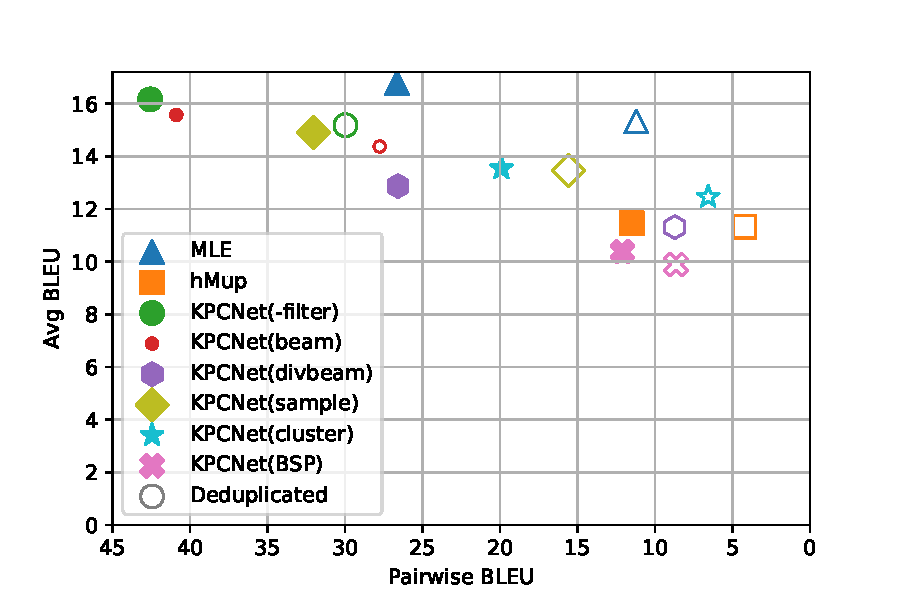
\includegraphics[width=\linewidth]{tradeoff-2BLEU.pdf}
  \caption{Group-level Automatic metrics on the whole test set of \texttt{Home \& Kitchen}. The lower Pairwise BLEU, the more diverse the generated group. Solid markers are the results for the top 3 candidates in the original group, while hollow markers measures the remaining 3 after deduplication. Points located near top-right are preferred as they achieve a good tradeoff between the 2 metrics.}
  \label{fig:group-filter}
  \end{figure}

  

\subsubsection{Group-level Evaluation}



The group-level automatic evaluation metrics before and after deduplication for each system are shown in Figure \ref{fig:group-filter}. Original results are shown in solid markers. KPCNet(BSP) has the poorest Avg BLEU and we found the results very likely to be ungrammatical and illogical, and we thus omit it in the following evaluation. hMup has the highest local diversity while has the second poorest Avg BLEU. MLE has moderate level of local diversity and the highest Avg BLEU, and we found that Keyword Filtering slightly harmed Avg BLEU, which is against our intuition. But we later found Avg BLEU doesn't correlate well with most human judgements (discuss later). Several diversity-promoting variants of KPCNet improved local diversity at the cost of Avg BLEU, among which KPCNet(cluster) achieved a best tradeoff between the two. Comparing the original and deduplicated results (hollow markers), we can see that our simple heuristic can effectively eliminate redundancy at the cost of slight degradation of Avg BLEU, as only nearly identical hypotheses with high BLEU are excluded. 

Group-level human evaluation results are shown in Table \ref{tab:group-human-eval}. We can see that all KPCNet variants clearly outperform baselines in \textit{Relevant} and \textit{Specific} while have a competitive performance in \textit{New info}. MLE rated best for \textit{Logical} for its conservative generations (low \textit{Specific}), and the questions tend to overlap with each other, as is reflected in high \textit{\#Redundant}. KPCNet(beam) has a even higher redundancy since its searching space is further limited by the conditioned keyword set. Diverse generation variants can help overcome this drawback. Especially, KPCNet(cluster) achieved the best \textit{\#Useful}, \textit{Avg Rank}, and its performance on all metrics is among the best of KPCNet variants. This shows that the semantically-coherent keyword sets produced by clustering can effectively improve the generation diversity and quality of KPCNet. 

We also study the system-level Pearson correlation between the automatic metrics and human judgements. Pairwise-BLEU has a correlation  of 0.915 with \textit{\#Redundant} ($p<0.01$), -0.835 with \textit{\#Useful} ($p<0.05$). Avg BLEU is shown only correlates well with \textit{Logical} (correlation: 0.849, $p<0.05$). This result validates the use of Pairwise-BLEU as an automatic proxy metric for local diversity.

\subsubsection{Case Study}

\begin{table*}[htbp]
  \centering
  \begin{tabular}{c|lcc}
      \hline
      product & \makecell[l]{homelegance 2588s accent dining chair, blue grey, set of 2} & {} & {} \\
      \hline
      \makecell[c]{system \\ (\#Useful)} & generation group & specific & problem \\
      \hline
      \makecell[c]{ref \\ (3)} & \makecell[l]{can any of the recent reviewers confirm the seat height ? \\ i see the question was posted in april ... \\ would u please send me the box dimensions ( when buy in \\ a set of 2 ) and the weight ? \\ can someone please tell me the depth of the chair seat \\ from the end of the curved back to the end of the seat ? } & \makecell[c]{2 \\ \\ 3 \\ \\ 3 \\ \\} & {} \\
      \hline
      \makecell[c]{MLE \\ (1)} & \makecell[l]{what is the seat height ? \\ what are the dimensions of the chair ? \\ what are the dimensions ?} & \makecell[c]{2 \\ 2 \\ 1} & {} \\
      \hline
      \makecell[c]{hMup \\ (1)} & \makecell[l]{what is the weight limit for the chair ? \\ i have a table that is a [UNK]. will this chair be able \\ to fit on a table ? \\ is this a set of 2 chairs or just one ?} & \makecell[c]{2 \\ 2 \\ \\ 2} & \makecell[c]{ \\ illogical \\ \\ repetitive} \\
      \hline
      \makecell[c]{KPCNet \\ (2)} & \makecell[l]{what is the \textbf{color} of the \textbf{chair} ? \\ what are the \textbf{dimensions} of the \textbf{seat} ? \\ what is the \textbf{weight} limit ? } & \makecell[c]{2 \\ 2 \\ 2} & \makecell[c]{ repetitive \\ \\  \\ } \\
      \hline
      \end{tabular}
      \caption{\label{table:quality} Example generation group and the human judgements for each system. Here we use KPCNet to stand for KPCNet(cluster) for brevity, and the appeared keywords of KPCNet are in bold. }
\end{table*}

\begin{table}[htbp]
  \small
  \centering
  \begin{tabular}{l|l}
  \hline
  Product & \makecell[l]{Novaform memory foam comfort curve pillow} \\
  \hline
  \makecell[l]{KPCNet \\ (cluster)} & \makecell[l]{is this a \textbf{firm} \textbf{pillow}? (pillow, foam, sleep, firm) \\ is this pillow good for \textbf{stomach sleepers}? \\ (stomach, sleeper)} \\
  \hline
  Product & \makecell[l]{full-sized headboard in solid wood} \\
  \hline
  \makecell[l]{KPCNet \\ (cluster)} & \makecell[l]{what is the height of this \textbf{headboard} ? \\ (bed frame headboard) \\ does it have a \textbf{box spring} ? (mattress box spring)} \\
  \hline
  \end{tabular}
  \caption{\label{tab:kwd-cluster} Example generation groups for KPCNet(cluster). Keywords in the parentheses.}
  \end{table}


Table \ref{tab:kwd-cluster} provides 2 example generation groups of KPCNet(cluster). For each group, the 6 predicted keywords captured specific aspects of the product. Then they are divided into 2 coherent groups (as they formed natural phrases such as ``firm pillow'' and ``stomach sleeper'') by clustering. Finally, the different conditioned keyword sets are reflected in the generation. In the first case, specific and diverse generations are successfully produced with precisely predicted keywords. We can see that the separation of keywords as controlling factors allows the novel use of classical clustering technique to help generate high-quality question groups by first producing coherent keyword sets. There are also bad cases like the second question in another group. The possible reason is that keyword predictor produced related but unsuitable keywords ``box spring'', which can be asked for a whole bed but not for headboard alone. This shows that predictor is the performance bottleneck of KPCNet.


We provide a group-level evaluation example in Table \ref{table:quality}. We can see that the diversity of MLE is very limited (it gets \textit{\#Useful} of only 1, though all 3 questions are valid, and thus \textit{\#Redundant} is 2), and it produces highly generic question. The generations are more diverse for hMup. However, we find that a certain expert of hMup has a style of long and illogical generation, like the second one demonstrated here. (It's abnormal to put chairs \textit{on} a table, and the text is not coherent as it doesn't use a pronoun in the second sentence.) This may attribute to its focus on \textit{style} instead of aspects of the products, as it is originally proposed for translation of diverse styles. This significantly harms hMup's group-level performance (Table 4) compared to its best single model (Table 3). KPCNet(cluster) produces a diverse and specific generation, and we can clearly see the effect of keyword in its generation. 

\subsection{\texttt{Office} Dataset Results}

For brevity, we only show the individual-level automatic evaluation and group-level human judgement results. All the experimental settings are the same with the previous experiments, except that we apply no keyword filtering here. 

\begin{table}[htbp]
  \centering
  \small
  \begin{tabular}{l|ccccc}
  \hline
  {} & Distinct-3 & BLEU & METEOR \\
  \hline
  ref  &        75.54 &        - &    - \\
  \hline
  MLE &        20.33 &  \textbf{14.73} & 13.81 \\
  hMup &        15.31 &  10.45 &    12.52  \\
  KPCNet &        \textbf{30.99} &     13.84 &    \textbf{15.29}  \\
  \hline
  \end{tabular}
  \caption{\label{tab:ind-auto-eval-office} Individual-level automatic evaluation results on the \texttt{Office} dataset.}
\end{table}

  
\begin{table*}[htbp]
\centering
\small
\begin{tabular}{l|ccccccc}
\hline
{} & Grammatical\tiny{[0-1]} & Relevant\tiny{[0-1]} & Logical\tiny{[0-1]} & New Info\tiny{[0-1]} & Specific\tiny{[0-4]} & \#Useful\tiny{[0-3]} & \#Redundant\tiny{[0-2]} \\
\hline
ref         &       0.993 &    0.997 &   0.993 &    0.933 &    2.713 &   2.420 &      0.330 \\
\hline
MLE         &       0.970 &    0.843 &   \textbf{0.883} &    0.797 &    1.470 &   1.070 &      0.420 \\
KPCNet &       \textbf{0.993} &    \textbf{0.940} &   0.817 &    \textbf{0.803} &    \textbf{1.903} &   \textbf{1.470} &      \textbf{0.190} \\
\hline
\end{tabular}
\caption{\label{tab:group-human-eval-office} Group-level human judgments on 100 samples from the \texttt{Office} dataset. KPCNet here uses keyword clustering.}
\end{table*}

Table \ref{tab:ind-auto-eval-office} shows that KPCNet still outperforms MLE in Distinct-3 and METEOR, while falls behind at BLEU. Both the automatic metrics and our manual check indicate that hMup fails to give comparable results for 
the small dataset, so we exclude it in group-level evaluation. 



Table \ref{tab:group-human-eval-office} shows that the performance of both models degraded here possibly due to the smaller data size. However, the observation is similar. KPCNet(cluster) outperforms MLE in most metrics especially at \textit{Relevant}, \textit{Specific} and \textit{\#Useful} despite a weakness at \textit{Logical}. This shows that KPCNet(cluster) can consistently improve the diversity and specificity of the generation.



\section{Related Work}
\paragraph{Clarification Question Generation} The concept of CQ can be naturally raised in a dialogue system where the speech recognition results tend to be erroneous so that we raise CQs for sanity check \citep{stoyanchev2014towards}, or the intents for a task is incomplete or ambiguous in a first short utterance and further CQs are needed to fill in the slots \citep{dhole2020resolving}. The concept is then extended to IR to clarify ambiguous queries \citep{aliannejadi2019asking}, and has been successfully put into practice \citep{zamani2020generating}. Other application areas including KBQA \citep{xu2019asking} and open-domain dialogue systems \citep{aliannejadi2020convai3}. CQGen can also be applied to help refine posts on websites like StackExchange \citep{Kumar_2020} and Amazon \citep{rao2019answer}. In this context, our work closely follows the research line of \citep{rao2018learning, rao2019answer, cao2019controlling}. \citet{rao2018learning} first adopted a retrieval-then-rank approach. They \citep{rao2019answer} then proposed a generation approach to train the model to maximize the utility of the hypothetical answer for the questions with GAN, to better promote specificity. \citet{cao2019controlling} propose to control the specificity by training on data with explicit indicator of specificity, but it requires additional specificity annotation. Towards the similar specificity goal, we adopted a different keyword-based approach. They also assume generating one question per context, which we claim is not sufficient to cover various possible information needs, and thus propose the task of the diverse CQGen.

\paragraph{Diverse Generation} The demand for diverse generation exists in many other fields~\cite{vijayakumar2018diverse, LiangZ18code, shen2019mixture}, and we've drawn inspirations from these literatures. For image captioning, we may use multiple descriptions for different focusing points of a scene. \textit{Diverse Beam Search} \citep{vijayakumar2018diverse} was proposed to broaden the searching space to catch such diversity by dividing groups in decoding and imposing repetition penalty between them. For machine translation, a context can be translated with different styles. \citet{shen2019mixture} thus proposed \textit{Mixture of Expert} models including hMup to reflect various styles with a discrete latent variable (\textit{expert}). And here for CQGen, diversity is required to cover various potentially missing aspects, so we come up with the idea to use keywords as a controlling variable like \textit{expert} to promote diversity.


\section{Conclusion}

In this paper, we incorporated the idea of Cookie Theft picture description task into the evaluation of the high-level cognitive abilities of LVLMs and designed a novel evaluation benchmark called CogBench.
% Images in CogBench are of high quality and require more cognitive reasonings to understand, which makes it different from existing image datasets.
The images in CogBench are of high quality and demand more complex cognitive reasoning for interpretation, setting it apart from existing image datasets.
% It consists of a image description task and a VQA task.
Experiments show that there is still a large gap between the cognitive abilities of LVLMs and human beings, indicating CogBench is a challenging benchmark.

% In the future


\begin{acks}
This work was partly supported by the
SJTU-CMBCC Joint Research Scheme and SJTU Medicine-Engineering
Cross-disciplinary Research Scheme.
%To Robert, for the bagels and explaining CMYK and color spaces.
\end{acks}

%%
%% The next two lines define the bibliography style to be used, and
%% the bibliography file.
\bibliographystyle{ACM-Reference-Format}
\bibliography{cqgen}

%%
%% If your work has an appendix, this is the place to put it.
\appendix

\section{Depression Templates}

\begin{table}[htbp]
  \small
  \centering
  \begin{tabular}{l|l}
  \hline
  Dimension & Template \\
  \hline
  Feeling Depressed  &  I feel depressed. \\
  Diagnosis &  I am diagnosed with depression. \\
  Treatment &  I am treating my depression. \\
  \hline
  Sadness & I feel sad.  \\
  Pessimism & I am discouraged about my future.  \\
  Past Failure & I always fail. \\
  Loss of Pleasure & I don't get pleasure from things. \\
  Guilty Feelings & I feel quite guilty. \\
  Punishment Feelings & I expected to be punished. \\
  Self-Dislike & I am disappointed in myself. \\
  Self-Criticalness & I always criticize myself for my faults. \\
  Suicidal Thoughts or Wishes & I have thoughts of killing myself. \\
  Crying & I always cry. \\
  Agitation & I am hard to stay still. \\
  Loss of Interest & It's hard to get interested in things. \\
  Indecisiveness & I have trouble making decisions. \\
  Worthlessness & I feel worthless. \\
  Loss of Energy & I don't have energy to do things. \\
  Changes in Sleeping Pattern & I have changes in my sleeping pattern. \\
  Irritability & I am always irritable. \\
  Changes in Appetite & I have changes in my appetite. \\
  Concentration Difficulty & I feel hard to concentrate on things. \\
  Tiredness  & I am too tired to do things. \\
  Loss of Interest in Sex & I have lost my interest in sex. \\
  \hline
  \end{tabular}
  \caption{The main templates and their corresponding dimensions we used in our experiments, including 3 direct depression descriptions and 21 indirect symptoms derived from BDI-II \citep{beck1996beck}. }
  \label{table:bdi}
\end{table}


We provide the complete templates in Table \ref{table:bdi}. We mainly use a combination of 3 direct depression descriptions and the 21 indirect symptoms derived from BDI-II. We also experimented other well-known depression scales like HDRS \citep{hamilton1986hamilton}, CES-D \citep{Lenore1977CES-D} and PHQ-9 \citep{kroenke2001phq} (We will release our revised templates for theses scales along with our code). The original scales usually contain different descriptions under the same dimension to distinguish different level of intensity or frequency. However, we find that current sentence representations have difficulty in capturing such nuanced differences. We thus condense the descriptions of each dimension into one general template (A few may have more, if there are significant intra-dimension difference).


\end{document}
\endinput
%%
%% End of file `sample-sigconf.tex'.
